\documentclass[10pt]{article}
%\usepackage{C:/Users/zhaor/MASTER/UNIVERSITY/NotesTeX/NotesTeX} %/Path/to/package should be replaced with package location
\usepackage{/Users/zhaor/MASTER/UNIVERSITY/NotesTeX/NotesTeX} %/Path/to/package should be replaced with package location
\usepackage{esvect}
\usepackage{cancel}
\usepackage{lipsum}
\usepackage{float}
\graphicspath{ {./images/} }

\title{{\Huge PHY294 - Quantum and Thermal Physics}\\{\Large{Grade 12 quantum chem on steroids}}}
\author{Regis Zhao\footnote{\href{https://google.com/}{\textit{TeX file on GitHub}}}}

\affiliation{University of Toronto}
\emailAdd{regis.zhao@mail.utoronto.ca}

\begin{document}

\maketitle
\flushbottom
\newpage

\pagestyle{fancynotes}



\part{Quantum Physics}

\section{The 3D Schrodinger Equation}

\subsection{The 3D Schrodinger Equation}
In 3D, the wave function $\psi$ depends on all three spatial coordinates, i.e. $\psi = \psi(x, y, z) = \psi(\mathbf{r})$, where $\mathbf{r}$ is the position vector. Similarly the potential energy will also depend on $x$, $y$, and $z$, i.e. $U = U(x, y, z) = U(\mathbf{r})$. Then the Schrodinger equation looks like:
\begin{definition}
    \textbf{The 3D Schrodinger Equation}:
    \begin{align}
        \frac{\partial^2 \psi}{\partial x^2} + \frac{\partial^2 \psi}{\partial y^2} + \frac{\partial^2 \psi}{\partial z^2} = \frac{2M}{\hbar^2} [U - E] \psi
    \end{align}
\end{definition}

\subsection{2D Square Box}
Before considering 3D systems, we look at an example of calculating $\psi$ and allowed energies in 2D. In particular, we look at solving the Schrodinger equation for a particle in a 2D square box, analagous to a puck sliding on a frictionless surface surrounded by walls.

The Schrodinger equation in 2D:
\begin{align}
        \frac{\partial^2 \psi}{\partial x^2} + \frac{\partial^2 \psi}{\partial y^2}  = \frac{2M}{\hbar^2} [U - E] \psi
\end{align}

The method for solving the Schrodinger equation depends what the potential energy function $U(\mathbf{r})$ is. In the case of a particle in a 2D square box, the particle can never travel outside, so the potential energy outside of the box is infinity, and the potential energy inside is 0, so all of its energy is kinetic:
\begin{align}
    U(x,y) =
    \begin{cases}
        0 & \text{when $0 \leq x \leq a$ and $0 \leq y \leq a$} \\ 
        \infty & \text{otherwise}
    \end{cases}
\end{align}

To find the possible energies for this quantum system, we solve the Schrodinger equation with the above potential energy function. Since $U = 0$ inside the box, the Schrodinger equation becomes
\begin{align}
        \frac{\partial^2 \psi}{\partial x^2} + \frac{\partial^2 \psi}{\partial y^2}  = \frac{2ME}{\hbar^2} \psi
\end{align}
for all $x$ and $y$ inside the box. Regarding the boundary conditions, since the particle can't escape from the box, $\psi(x, y)$ must be zero outside the box, and since $\psi(x, y)$ must be continuous, it must be zero on the boundary as well.  

\subsubsection{Finding $\psi$ using Separation of Variables}
We solve the Schrodinger equation (which is a differential equation) by separation of variables, i.e. we try to find a solution with the form: 
\begin{align}
    \psi(x, y) = X(x)Y(y)
\end{align}
To see if the Schrodinger equation has solutions of the above form, we substitute this "test" solution into Schrodinger's equation. First we simplify the partial derivatives:
\begin{align}
    \frac{\partial^2 \psi}{\partial x^2} = Y(y)X''(x) \\
    \frac{\partial^2 \psi}{\partial y^2} = X(x)Y''(y)
\end{align}
Substituting these into the Schrodinger equation:
\begin{align}
    Y(y)X''(x) + X(x)Y''(y) = - \frac{2ME}{\hbar^2}X(x)Y(y)
\end{align}
Dividing both sides by $X(x)Y(y)$:
\begin{align}
    \frac{X''(x)}{X(x)} + \frac{Y''(y)}{Y(y)} = - \frac{2ME}{\hbar^2}
\end{align}
Rearranging this equation, we get
\begin{align}
    \frac{X''(x)}{X(x)} = - \frac{2ME}{\hbar^2} - \frac{Y''(y)}{Y(y)}
\end{align}
This equation implies that a function of $x$ doesn't depend on $x$, which implies that the function is a constant, i.e.
\begin{align}
    \frac{X''(x)}{X(x)} = \text{constant}
\end{align}
Referring to this constant as $-k_x^2$, we can rearrange the above equation:
\begin{align}
    X''(x) = -k_x^2 X(x)
\end{align}
This equation itself is a differential equation that we already know the solution to:
\begin{align}
    X(x) = B \sin k_x x
\end{align}
where B is a constant. To satisfy the boundary conditions (that $X(0)=X(a) = 0$), we find that $k_x$ must be an positive integer multiple of $\pi/a$, i.e.
\begin{align}
    k_x = \frac{n_x \pi}{a}
\end{align}
Therefore,
\begin{align}
    X(x) = B \sin \frac{n_x \pi x}{a}
\end{align}

Following the same logic, we find that
\begin{align}
    Y(y) = C \sin \frac{n_y \pi y}{a}
\end{align}

Combining these two solutions, the complete wave function is given by 
\begin{gather}
    \psi(x, y) = X(x)Y(y) = BC \sin k_x x \sin k_y y \\
    \psi(x, y) = A \sin \frac{n_x \pi x}{a} \sin \frac{n_y \pi y}{a}
\end{gather}

\subsubsection{Finding Allowed Energies}
Recall that 
\begin{align}
    \frac{X''(x)}{X(x)} + \frac{Y''(y)}{Y(y)} = - \frac{2ME}{\hbar^2}
\end{align}
We now know that $X''/X$ is equal to $-k_x^2$ which is equal to $n_x \pi /a$. Similar logic follows for $Y''/Y$. Substituting this into the above equation, we get
\begin{align}
    - \frac{n_x^2 \pi^2}{a^2} - \frac{n_y^2 \pi^2}{a^2} = - \frac{2ME}{\hbar^2}
\end{align}
Solving for E, we find the allowed energy values:
\begin{align}
    E = E_{n_x, n_y} = \frac{\hbar^2 \pi^2}{2Ma^2} (n_x^2 + n_y^2)
\end{align}



\subsection{Energy Levels of the Hydrogen Atom}
The energy of a state is given by:
\begin{align}
    E = - \frac{E_R}{n^2}
\end{align}

\section{Electron Spin}

\subsection{Spin Angular Momentum}
The angular momentum of an electron is the sum of two terms:
    \begin{align}
        \mathbf{J} = \mathbf{L} + \mathbf{S}        
    \end{align}
where $\mathbf{L}$ is the orbital angular momentum and $\mathbf{S}$ is the electron's \textbf{spin}. The magnitude of $\mathbf{L}$ is given by:
\begin{align}
     L = \sqrt{l(l+1)}\hbar
\end{align}
The magnitude of $\mathbf{S}$ is given by a similar formula:
\begin{align}
    S = \sqrt{s(s+1)}\hbar
\end{align}
The difference is that while $l$ can take on integer values, $s$ always has a fixed value for an electron: \sn{Some other elementary particles have different values for $s$}
\begin{align}
    s = \frac{1}{2}    
\end{align}
Therefore electron spin always has the same magnitude, and is sometimes called the \textit{intrinsic angular momentum}:
\begin{align}
    S = \frac{\sqrt{3}}{2}\hbar 
\end{align}
Recall that the z-component of $\mathbf{L}$ is given by
\begin{align}
    L_z = m\hbar
\end{align}
where $m$ can take on integer values from $-l$ to $l$. Similarly, for the z-component of spin: 
\begin{align}
    S_z = m_s\hbar    
\end{align}
where $m_s$ is the fourth quantum number that takes on integer values from $-s$ to $s$. But since $s = \frac{1}{2}$, $m_s$ only has two possible values:
\begin{align}
    m_s = \pm \frac{1}{2}
\end{align}
and therefore
\begin{align}
    S_z = \pm \frac{1}{2}\hbar
\end{align}
These two possibilities are referred to as "spin up" or "spin down", also represented by arrows pointing up or down. \sn{$\mathbf{S}$ is never actually parallel to the z-axis though (since $S_z$ is smaller than $S$)}.

Complete specification of an electron's state of motion requires specification of both its orbital motion (defined by quantum numbers $n$, $l$, $m$) \textit{and} spin orientation (defined by $m_s$) -- requires all 4 quantum numbers to specify its \textbf{quantum state}. 

For Hydrogen, its energy is almost completely independent of spin orientation. For the $n^{th}$ energy level, there are $n^2$ possible values of $l$ and $m$. For each of these values, there are also two possible spin orientations. Therefore:
\begin{align}
    \text{degeneracy of $n^{th}$ level in \textbf{hydrogen}} = 2n^2
\end{align}

The electron is entirely elementary -- not made of any other particles. Therefore, its spin is not dependent of anything else -- it is an intrinsic property of the electron.



\subsection{Magnetic Moments}
Most evidence for electron's spin angular momentum relates to the magnetic moment associated with rotating electric charge. 

Consider an electron orbiting a nucleus. This small orbiting charge is essentially a small current loop. Current loops produce magnetic fields which respond to externally applied magnetic fields.

We use $\mathbf{A}$ to represent a vector perpendicular to the plane of the loop. 

\begin{align}
    \mathbf{\Gamma} = i\mathbf{A} \times \mathbf{B} \\
    \mathbf{\Gamma} = \boldsymbol{\mu} \times \mathbf{B}
\end{align}
where $\boldsymbol{\mu} = i \mathbf{A}$ is the \textbf{magnetic moment} of the loop. An applied magnetic field $\mathbf{B}$ exerts a torque $\mathbf{\Gamma}$ on the current loop that tries to align the magnetic moment $\boldsymbol{\mu}$ with $\mathbf{B}$. Due to this torque, if the magnetic moment of a current loop in a magnetic field isn't aligned with the field, it stores potential energy $U$, given by
\begin{align}
    U = -\boldsymbol{\mu} \cdot \mathbf{B}
\end{align}
We can relate magnetic moment $\mu$ to angular momentum $L$ in a ratio: \sn{Both $\mu$ and $L$ are a result of the electron's orbital motion. Some math is skipped here lol.} \sn{This ratio is called the \textbf{gyromagnetic ratio}. It is constant -- only depends on the charge and mass of the electron.}
\begin{align}
    \frac{\mu}{L} = \frac{e}{2m_e}    
\end{align}
Since electron charge is negative, the current flows in the opposite direction of the electron's velocity, and therefore $\mu$ and $L$ point in opposite directions. So we can rewrite the above ratio:
\begin{align}
    \boldsymbol{\mu} = -\frac{e}{2m_e} \mathbf{L}
\end{align}
Since in quantum mechanics, angular momentum $\mathbf{L}$ is quantized (just $2l+1$ possible orientations), then the magnetic moment $\boldsymbol{\mu}$ is also quantized with $2l + 1$ possible orientations.

Note that the above equation only gives the magnetic moment due to the \textit{orbital} motion of an electron. Magnetic moment arises from an electron's spinning motion as well, but first we'll look at cases where the magnetic moments due to spin cancels out.



\subsection{The Zeeman Effect}
Due to electron motion, most atoms have a magnetic moment. When you apply a magnetic field, you apply torque and change the atom's potential energy -- you change the atom's energy levels by $U = -\boldsymbol{\mu} \cdot \mathbf{B}$. This changes the energy of photons emitted/absorbed, therefore changing the spectrum. This is the \textbf{Zeeman Effect}.

We first look at cases where magnetic moments due to electron spin cancel out. There are many states of helium where the spins of its two electrons point in opposite directions and therefore their magnetic moments cancel out; they produce only one spectral line and are therefore called \textbf{singlet states}. Also, in all states of helium, one of the electrons has zero orbital angular momentum. Therefore, in singlet states, the total magnetic moment of the state is just the
the magnetic moment due to the orbital motion of one of the electrons.

Without an applied magnetic field, for a given energy level, the angular momentum has $2l + 1$ different orientations that all have the same energy. Therefore the energy level is ($2l + 1$)-fold degenerate. 

After applying a magnetic field, the energy level of each of the $2l + 1$ orientations changes by $U = -\boldsymbol{\mu} \cdot \mathbf{B}$, therefore removing the ($2l + 1$)-fold degeneracy.

The size of the energy shift due to the magnetic field is given by: \sn{note that the energy shift is dependent on quantum number $m$; therefore it's often called the \textbf{magnetic quantum number}}
\begin{align}
    \Delta E = -\boldsymbol{\mu} \cdot \mathbf{B} \\
    \text{some math...} \\ 
    \Delta E = \left( \frac{e\hbar}{2m_e} \right) mB \\ 
    \Delta E = m \mu_B B
\end{align}
where we define
\begin{align}
    \mu_B = \frac{e\hbar}{2m_e} = 9.27 \cdot 10^{-24} A \cdot m^2
\end{align}
as the \textbf{Bohr magneton} (has the units of a magnetic moment).

Since $m$ can only take on consecutive integer values, we see that the energy separation of adjacent energy levels is equal to:
\begin{align}
    \text{separation of adjacent levels} = \mu_B B
\end{align}
We can also express $\mu_B$ in units of joules/tesla:
\begin{align}
    \mu_B = 5.79 \cdot 10^{-5} eV/T
\end{align}
We interpret this to mean: if you apply a 1 tesla magnetic field, it causes a separation of adjacent levels by $5.79 \cdot 10^{-5} eV$.

Note that we've only considered 

\subsection{Spin Magnetic Moments}
The magnetic moment of an electron due to its spinning motion is equal to
\begin{align}
    \boldsymbol{\mu_{spin}} = -\frac{e}{m_e} \mathbf{S}
\end{align}
The total magnetic moment of any electron is equal to the sum of its orbital and spin magnetic moments:
\begin{align}
    \boldsymbol{\mu_{tot}} = \boldsymbol{\mu_{orb}} + \boldsymbol{\mu_{spin}} = -\frac{e}{2m_e} (\mathbf{L} + 2\mathbf{S})  
\end{align}



\subsection{Anomalous Zeeman Effect}
Anomalous Zeeman Effect occurs when the spin magnetic moment don't cancel out as they did for the normal Zeeman Effect.

We look at a hydrogen atom in a state with zero orbital angular momentum (in the $s$ state, with $l = 0$). Therefore only the spin angular momentum contributes to the magnetic moment. 

When we apply a magnetic field $\mathbf{B}$, the energy shift is
\begin{align}
    \Delta E = \pm \mu_B B
\end{align}
If the electron is spin up, its energy is raised; if it's spin down, its energy is lowered. Therefore the separation between the two levels is
\begin{align}
    \text{separation of adjacent levels} = 2 \mu_B B
\end{align}



\section{Multielectron Atoms}
Unlike the Bohr model, the Schrodinger equation is able to predict the properties of multielectron atoms and moleculues.

\subsection{The Independent-Particle Approximation}
For two or more electrons, there is no exact solution to the Schrodinger equation -- only approximations. The \textbf{independent particle approximation} (IPA) is the basis for most calculations of multielectron atoms. 

Essential feature of IPA: each electron is considered to move independently in a field of the other $Z-1$ electrons and the nucleus. Furthermore we can assume the distribution of the other $Z-1$ electrons is spherically symmetric around the nucleus. \sn{For this reason, the IPA is sometimes called the central-field approximation} Therefore the charge distribution seen by any one electron is spherically symmetric, meaning that the IPA potential energy is only a function
of $r$, i.e. $U(r)$.

First, if an electron is \textit{outside} a spherical distribution of total charge $Q$, the force experienced by the electron is the same force as if $Q$ was a point charge at $r = 0$:
\begin{align}
    F = k \frac{Qe}{r^2}
\end{align}
Second, if the electron is \textit{inside} a spherical shell of charge, it experiences no force from the shell at all.

So, if the electron is close enough to the nucleus, it will be inside all the other electrons -- the only force it experiences is the force from the nuclear charge $Ze$:
\begin{align}
    F = \frac{Zke^2}{r^2}
\end{align}
If the electron is outside all other electrons, the force it experiences is:
\begin{align}
    F = \frac{ke^2}{r^2}    
\end{align}

The potential energy $U(r)$ of the electron is the integral of the force. It is given by
\begin{align}
    U(r) = -Z_{eff}(r) \frac{ke^2}{r}    
\end{align}
where $Z_{eff}(r)$ is the \textbf{effective charge} felt by the electron. When $r$ is inside the other electrons:
\begin{align}
    Z_{eff} \approx Z
\end{align}
When $r$ is outside the other electrons:
\begin{align}
    Z_{eff} \approx 1
\end{align}



\subsection{IPA Energy Levels}
The ground state energy of the innermost electron ($1s$) is approximately
\begin{align}
    E_{1s} \approx -Z^2 E_R
\end{align}

In hydrogen, all orbitals with the same principle quantum number $n$ have the same energy and therefore all states with the same $n$ are degenerate (degeneracy of $n^2$). In multielectron atoms, states with smaller $l$ values penetrate closer to the nucleus and are lower in energy and therefore remove the degeneracy between the different orbital types. In multielectron atoms, only states of the same orbital types are degenerate, with a degeneracy of $2(2l+1)$.

The clustering of electrons into spatial shells occurs in multielectron atoms. The most probable radius of these shells is roughly
\begin{align}
    r_{mp} \approx \frac{n^2 a_B}{Z_{eff}}    
\end{align}

\subsection{The Pauli Exclusion Principle}
\begin{theorem}
    \textbf{Pauli Exclusion Principle}: No two electrons in a quantum system can occupy the same quantum state. 
\end{theorem}
Note that the Pauli exclusion principle applies to other particles as well, not just electrons.




\newpage
\part{Thermal Physics}
Thermal physics is a combination of Thermodynamics and Statistical Mechanics. We will focus on statiscal mechanics.

\section{Lecture 1 -- Ideal Gas Law}
\begin{itemize}
    \item what is temperature? The thing that's measured by thermometers
    \item Types of thermometers:
        \begin{itemize}
            \item Mercury bulb: Expansion of mercury
            \item Bi-metallic Strip: Different metals expand differently
            \item IR Thermometer: Infrared spectrum depends on temperature
            \item Thermistor: resistance depends on temperature
            \item Gas bulb Thermomemter: Pressure depends on temperature
        \end{itemize}
\end{itemize}
How the gas bulb thermometer works:
\begin{itemize}
    \item Ideal gas law:
    \begin{align}
        P = kT \frac{N}{V} \\
        P = RT \frac{n}{V} \\
        kN = Rn
    .\end{align} 
    \item assume that gas molecules bounce elastically off of the walls of the gas container
    \item for simplicity: igonore collisions between molecules
    \item therefore we can treat one particle at a time
    \item consider a particle in a box at speed $v$ -- $x$ component is $v_x$
    \item in an elastic collision, the $x$ component simply changes sign
    \item the pulse force the particle exerts on the wall during a bounce is:
    \begin{align}
        F_x = m \frac{\Delta v_x}{\Delta t_c} = m \frac{2v_x}{\Delta t_c}
    .\end{align}
\item let's take the average force:
    \begin{align}
        \overline{F_x} = m \frac{2v_x}{\Delta t} \\ 
        \Delta t = \frac{2L}{v_x} \\ 
        \overline{F_x} = \frac{mv_x^2}{L}
    .\end{align}
\item Pressure for one particle can be given by:
    \begin{align*}
        P = \frac{\overline{F_x}}{A} \\ 
        P = \frac{mv_x^2}{V}
    .\end{align*}
\item Pressure for $N$ particles:
    \begin{align*}
        P = \sum_{i=1}^{N} \frac{mv_{x,i}^2}{V} = \frac{m}{V} \sum_{i=1}^{N} v_{x,i}^2
    .\end{align*}
\end{itemize}
\begin{theorem}
    \textbf{Kinetic Theory}
    \begin{align*}
        P = \frac{m \overline{v^2}}{3} \frac{N}{V}
    .\end{align*}
\end{theorem}
\begin{itemize}
    \item comparing this result to the ideal gas law:
    \begin{align*}
        \frac{m\overline{v^2}}{3} = kT
    .\end{align*}
\item note that average kinetic energy per particle is
    \begin{align*}
        \overline{E} = \frac{m\overline{v^2}}{2}
    .\end{align*}
\item then we obtain:
    \begin{align*}
        T = \frac{m\overline{v^2}}{3k} = \frac{2\overline{E}}{3k}
    .\end{align*}
\end{itemize}

\begin{definition}
    \textbf{Temperature (for an ideal gas)}: For an ideal gas, temperature is a measure of the average kinetic energy per particle
    \begin{align*}
        T \equiv \frac{m\overline{v^2}}{3k} = \frac{2\overline{E}}{3k} \\
    .\end{align*}
    \begin{itemize}
        \item using this definition of temperature, we derived the \textbf{ideal gas law}  as well
            \begin{gather*}
                P = kT \frac{N}{V}
            .\end{gather*}
        \item experimentally this is what a thermometer measures
    \end{itemize}
    \begin{align*}
        \overline{E} = \frac{3}{2}kT
    .\end{align*}
\end{definition}


\section{Lecture 2 -- Equipartition}
\begin{itemize}
    \item how does this apply to things that aren't gases?
    \item can we say something about speed distribution?
    \item why do things come into thermal equilibrium?
    \item what does this have to do with the second law of thermodynamics?
\end{itemize}
\begin{itemize}
    \item What is the total energy $U$, in an ideal gas at temperature $T$?
    \begin{align*}
        U = N\overline{E} = 3 \frac{NkT}{2}
    .\end{align*}
\item so increasing $U$ increases $T$
\end{itemize}
\begin{definition}
    \textbf{Heat Capacity}: the energy required for a unit change in temperature
    \begin{align*}
        C_V \equiv \frac{\partial U}{\partial T} |_{V,N,\ldots} = \frac{3Nk}{2} = \frac{3nR}{2} \\ 
        C_V = \frac{3R}{2} \text{for 1 mole of an ideal gas}
    .\end{align*}
    \begin{itemize}
        \item recall that $Nk = nR$
        \item for an Ideal Gas (theory): $C_v = 12.47 \frac{J}{K \cdot mol}$
    \end{itemize}
\end{definition}

\begin{theorem}
    \textbf{Equipartition Theorem}: At temperature $T$, the average energy of any quadratic degree of freedom is $\frac{1}{2}kT$, i.e.
    \begin{gather*}
            U = D \frac{kT}{2} \\ 
            U = \frac{dNkT}{2} \\ 
            U = d \frac{nRT}{2}
    .\end{gather*}
    \begin{itemize}
        \item then the heat capacity:
    \end{itemize}
    \begin{gather*}
            C_V = \frac{dnR}{2}
    .\end{gather*}
    \begin{itemize}
        \item then for an ideal gas (which has 3 DOF per particle):
        \begin{gather}
            U = N\overline{E} = \frac{3}{2}Nmv^2 = 3N \frac{kT}{2}
        .\end{gather}
    \end{itemize}
\end{theorem}

\subsection{Rigid body quadratic degrees of freedom}
\begin{itemize}
    \item there are three translational degrees of freedom:
    \item and there are three rotational degrees of freedom:
    \begin{align*}
        E = \frac{1}{2}I\omega^2
    .\end{align*}
\item shouldn't there be 6 degrees of freedom?
\item Rotational Quantum Modes: monoatmoic molecules:
\item From quantum mechanics, the rotational energy levels for a rigid object are:
    \begin{align*}
        E_J = \frac{\hbar}{2I}J(J+1)
    .\end{align*}
\item for a solid sphere:
    \begin{align*}
        I = \frac{2}{5}mr^2
    .\end{align*}
\item in the case of an atom, $r$ is the radius of the nucleus -- where all the mass is
\item for Argon, treating the nucleus as a solid sphere, we get:
    \begin{align*}
        E_1 = 
    .\end{align*}
\item for monoatmoic molecules:
    \begin{itemize}
        \item the mass is ~all in the nucleus
        \item the moment of inertia is very very small
        \item the first excited rotational mode is at a high energy
        \item the first excited quantum mode is not excited at any sensible temperature (the modes are "frozen out")
        \item \textbf{monoatomic molecules only have 3 DOF} 
    \end{itemize}
\item For diatomic molecules:
    \begin{itemize}
        \item the mass is ~ all in the nuclei, which are separated by $~10^{-10}$ m
        \item Along the long (green) axis, it behaves the same as a monoatomic molecule (frozen rotational mode)
        \item the other two axes have much higher moments with very low energy rotational modes
        \item at low enough temperatures, these rotational modes will also be frozen out, but\ldots
        \item at room temperature, many modes are accessible, so the equipartition theorem applies to them
        \item \textbf{Diatomics have 5 degrees of freedom}  -- 3 translational and 2 rotational
    \end{itemize}
\end{itemize}

\subsubsection{Idealized Solids}
\begin{itemize}
    \item model a solid as atoms connected by springs
    \item 3 kinetic DOF per atom:
        \begin{align*}
            E = \frac{1}{2}mv^2
        .\end{align*}
    \item AND 3 potential DOF in the spring:
        \begin{align*}
            E = \frac{1}{2}k\Delta x^2
        .\end{align*}
    \item Total: $d = 6$
\end{itemize}
\subsubsection{$C_V$ vs  $C_P$}
Heat capacity at constant volume:
\begin{align*}
    C_V \equiv \frac{\partial U}{\partial T} 
.\end{align*}
\begin{itemize}
    \item hard to measure for solids since they tend to expand thermally
\end{itemize}
Heat capacity at constant pressure:
\begin{gather*}
    C_P \equiv \left. \frac{\partial U}{\partial T} \right|_P + P \left. \frac{\partial V}{\partial T} \right|_P
.\end{gather*}
\begin{itemize}
    \item first term is energy absorbed by the material
    \item second term is work done on the surrounding gas
\end{itemize}

\subsubsection{Summary}
\begin{itemize}
    \item equipartition theorem seems pretty powerful:
        \begin{itemize}
            \item predicts energy per mode as a function of temperature
            \item can be used to calculated a bunch of things
        \end{itemize}
    \item But:
        \begin{itemize}
            \item we didn't really prove it 
            \item it doesn't really work when quantum levels matter 
            \item it isn't always really clear that "degrees of freedom" are well defined 
            \item works in average energy, so only gives mean-squared values for speeds, etc.
            \item still don't know what entropy is 
            \item presumes but doesn't explain equilibrium
        \end{itemize}
\end{itemize}


\section{Lecture 3 -- Two State Systems}
\subsection{Statistics}
\subsubsection{Microstates and Macrostates}
\begin{itemize}
    \item \textbf{Microstate}: a specific configuration (e.g. HTH)
        \begin{itemize}
            \item all microstates are equally likely
        \end{itemize}
    \item \textbf{Macrostate}: defined by some combined quantities (e.g. 2H)
        \begin{itemize}
            \item may include many different microstates 
            \item not all macrostates are equally likely
        \end{itemize}
    \item \textbf{Multiplicity $\Omega$}: the number of microstates in a macrostate
        \begin{itemize}
            \item multiplicity is given by:
                \begin{align*}
                    \Omega (n) = {100 \choose n}
                .\end{align*}
            \item multiplicity of a two state system:
                \begin{align*}
                    \Omega(N,n) = {N \choose n}
                .\end{align*}
        \end{itemize}
    \item Probability of $n$ heads after $N$ coin flips:
        \begin{align*}
            P(N,n) = \frac{\Omega(N,n)}{\Omega_{tot}} = \frac{\Omega(N,n)}{2^N}
        .\end{align*}
    \item for 50 coins:
        \begin{figure}[h]
            \centering
            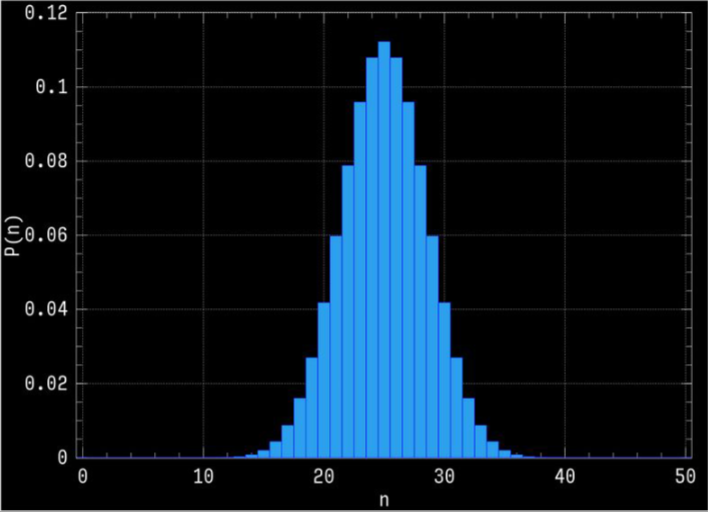
\includegraphics[width=0.8\textwidth]{probabilityDistributionCoins.png}
            \caption{Probability of $n$ coins flipped heads.}
            \label{fig:probabilityDistributionCoins}
        \end{figure}
\end{itemize}


\subsection{Paramagnets: an example of a two state system}
\begin{itemize}
    \item consider a system of $N$ little magnetic dipoles that can either point up or down relative to an externally applied magnetic field
    \item they don't influence each other
    \item external magnetic field applies a torque trying to align the dipoles with the field
    \item aligned has lower energy than unaligned
    \item ignoring the cost of energy: equal numbers of dipoles pointed up as down has a far higher probability
\end{itemize}


\section{Lecture 4 -- Einstein Solid}
\begin{itemize}
    \item model a solid as N independent harmonic oscillators
    \item the quantum energy levels for a harmonic oscillator are:
        \begin{align*}
            E = \left( q + \frac{1}{2} \right) \hbar \sqrt{\frac{k}{m}}  
        .\end{align*}
    \item so each oscillator has evenly spaced energy levels
        \begin{align*}
            E - E_o = q \hbar \sqrt{\frac{k}{m}} \\ 
            \implies E = q \hbar \sqrt{\frac{k}{m}} 
        .\end{align*}
    \item we don't really care about the ground state $E_o$ since it is constant, so we can ignore it
    \item each identical, independent oscillator can have exactly an integer quanta of energy
    \item imagine a system of 3 oscillators with a total of 2 quanta of energy 
    \item this energy can be distributed several different ways between the three oscillators
        \begin{figure}[h!]
            \centering
            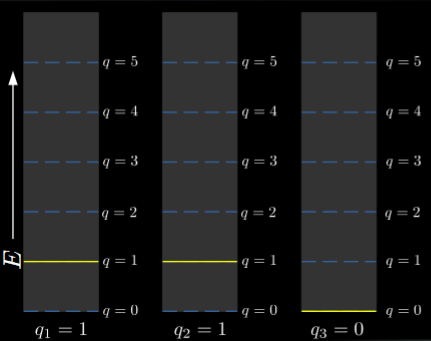
\includegraphics[width=0.8\textwidth]{quantumOscillatorArrangement}
            \caption{One possible arrangement of the three oscillators}
            \label{fig:quantumOscillatorsArrangement}
        \end{figure}
    \item the \textbf{microstate} is the exact configuration, e.g (0, 0, 2)
    \item the \textbf{macrostate} is the number of quanta of energy
    \item the \textbf{multiplicity} is the number of microstates that have this macrostate
    \item the multiplicity of the macrostate $q_{tot} = 2$ is:
        \begin{align*}
            \Omega(2) = 6
        .\end{align*}
    \item generally, \textbf{the multiplicity for $q$ quanta of energy distributed between $N$ oscillators} is:
        \begin{align*}
            \Omega(N,q) = {q+N-1 \choose q}
        .\end{align*}
    \item proof: we can draw configurations like this, where * is a quanta of energy and | separates the oscillators:
        \begin{figure}[h!]
            \centering
            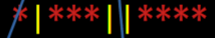
\includegraphics[width=0.8\textwidth]{multiplicityEinsteinProof}
            \caption{Representation of configuration of quanta of energy.}
            \label{fig:multiplicityEinsteinProof}
        \end{figure}
    \item so there are $q+N-1$ symbols, $q$ of which are a *
    \item $\Omega$ grows rapidly with $q$ and $N$, but grows more rapidly with $N$ (number of oscillators)
\end{itemize}

\subsubsection{Interaction of Einstein Solids}
\begin{itemize}
    \item imagine two Einstein solids:
        \begin{itemize}
            \item each with $N = 32$ oscillators
            \item $q_1 + q_2 = q_{tot} = 120$ quanta of energy distributed between them
        \end{itemize}
    \item how does $\Omega$ change with the distribution of $q_1$ and $q_2$?
    \item the multiplicity (number of different possible ways of arranging the quantas of energy) increases as you more evenly distribute the energy
    \item multiplicity of two solids:
        \begin{figure}[h]
            \centering
            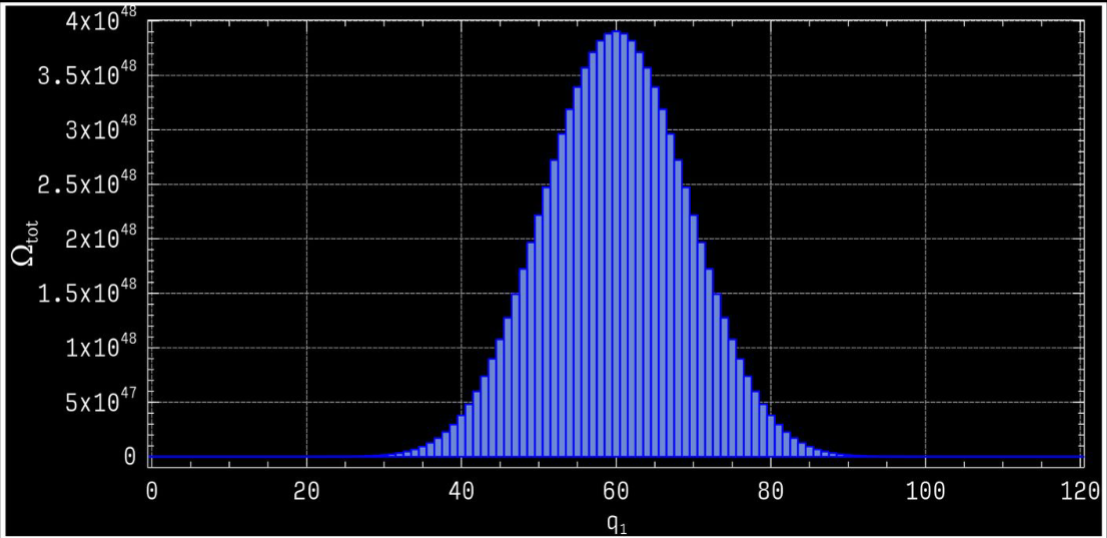
\includegraphics[width=0.8\textwidth]{multiplicityTwoSolids}
            \caption{Multiplicity of two interacting solids.}
            \label{fig:multiplicityTwoSolids}
        \end{figure}
    \item as you increase $N$ and $q$, the probability distribution becomes narrower -- the possibility of finding the microstates in an arrangement outside of the most probable one becomes lower and lower
    \item in real life, where there are huge numbers of atoms in solids, the probability distribution is extremely narrow -- much more likely to find system with evenly distributed energy
        \begin{figure}[h]
            \centering
            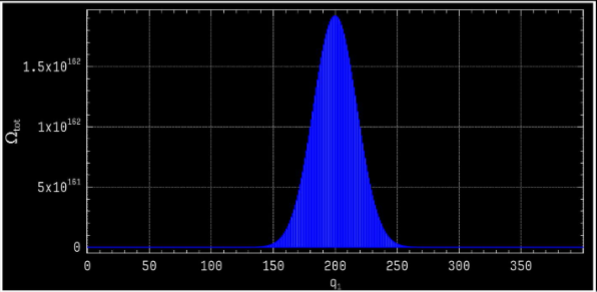
\includegraphics[width=0.8\textwidth]{multiplicityMoreNq}
            \caption{Mulitiplicity as you increase $N$ and $q$}
            \label{fig:mulitiplicityMoreNq}
        \end{figure}
    \item so if you imagine two Einstein solids:
        \begin{itemize}
            \item allow energy to flow between them freely
            \item assume that every accessible microstate is equally likely
        \end{itemize}
    \item therefore the probability that we will find the combined system in this macrostate is proportional to the multiplicity of the macrostate
    \item seems like this might be an explanation for thermal equilibrium\ldots
\end{itemize}


\section{Lecture 5 -- Large Numbers}
\begin{itemize}
    \item putting 2 einstein solids in thermal contact so that every microstate of the combined system is equally likely
    \item while each of the microstates of $ q_1 = 0$ are as likely as any other microstate, there are so few of them that we will never see it
    \item there are way more possible arrangements where the energy quanta are evenly split between the two materials
    \item dealing with real numbers (e.g. considering 1 mole of an Eintstein solid), numbers become extremely large and $\Omega$ becomes unreasonably large
\end{itemize}

\subsubsection{Dealing with (very) Large Numbers}
\begin{itemize}
    \item for \textit{large} numbers, you can ignore adding a small number to a large number (unless you later subtract)
    \item for \textit{very large} numbers, you can ignore multiplying by a large number (unless you later divide)
\end{itemize}

\begin{theorem}
    \textbf{Stirling's Approximation:} 
    \begin{align*}
        N! \approx \sqrt{2\pi N} {N \choose e}^N \quad \text{when $N \gg 1$}
    .\end{align*}
    \begin{itemize}
        \item this approximation is good to 0.8\% for $N = 10$ and around 0.03\% for $N = 300$
    \end{itemize}
    \begin{align*}
        \ln(N!) \approx N \ln(N) - N \quad \text{when $N\gg 1$}
    .\end{align*}
\end{theorem}

\subsection{Large N Multiplicity of Einstein Solids}
\begin{align}
    \Omega \approx \left( \frac{eq}{N} \right) ^N \; \text{when $q \gg N$ and} \; N \gg 1
\end{align}
\begin{itemize}
    \item for two Einstein solids:
\end{itemize}
\begin{align*}
    \Omega_1 \approx \left( \frac{eq_1}{N} \right) ^N \; \text{and} \; \Omega_2 \approx \left( \frac{eq_2}{N} \right) ^N \\ 
    \Omega_{tot} = \Omega_1 \Omega_2 = \left( \frac{e}{N} \right) ^{2N} (q_1 q_2)^N
.\end{align*}
\begin{itemize}
    \item the peak will be at $q_1 = q_2 = \frac{q}{2}$
    \item define $x = q_1 - \frac{q}{2} = \frac{q}{2} - q_2$ ($x$ is how far we are from the centre)
    \item then:
        \begin{align*}
            \Omega_{tot} = \left( \frac{e}{N} \right) ^{2N} \left[ \left( \frac{q}{2} \right) ^2 - x^2 \right] ^N \\ 
            \Omega_{tot} \approx \Omega_{max} \cdot e^{N(\frac{2x}{q})^2} \\ 
            \Omega_{max} = \left( \frac{e}{N} \right)^{2N} \left( \frac{q}{2}\right)^{2N}  
        .\end{align*}
\end{itemize}
\begin{figure}[h]
    \centering
    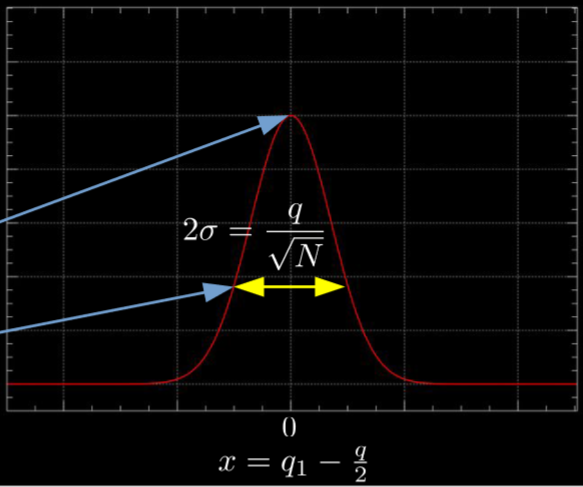
\includegraphics[width=0.8\textwidth]{multiplicityLargeNumbers}
    \caption{}
    \label{fig:multiplicityLargeNumbers}
\end{figure}
\begin{itemize}
    \item width of distribution is very very thin, but not zero:
        \begin{align*}
            \sigma = \frac{q}{2\sqrt{N} }
        .\end{align*}
    \item if $N = 10^{24}$ then $\sigma = \frac{q}{2 \cdot 10^{12}}$
\end{itemize}



\subsection{Introducing Entropy}
\begin{itemize}
    \item systems in thermal contact will tend to be found in states with the highest multiplicity $\Omega$
    \item \textbf{multiplicity increases}
    \item but dealing with numbers this big is a pain, so we introduce \textbf{entropy}:
         \begin{align*}
            S \equiv k \ln(\Omega)
        .\end{align*}
    \item systems in thermal contact will tend to be found in states with the highest entropy $S$
    \item \textbf{entropy increases}
    \item this is the \textbf{second law of thermodynamics}
        \begin{figure}[h]
            \centering
            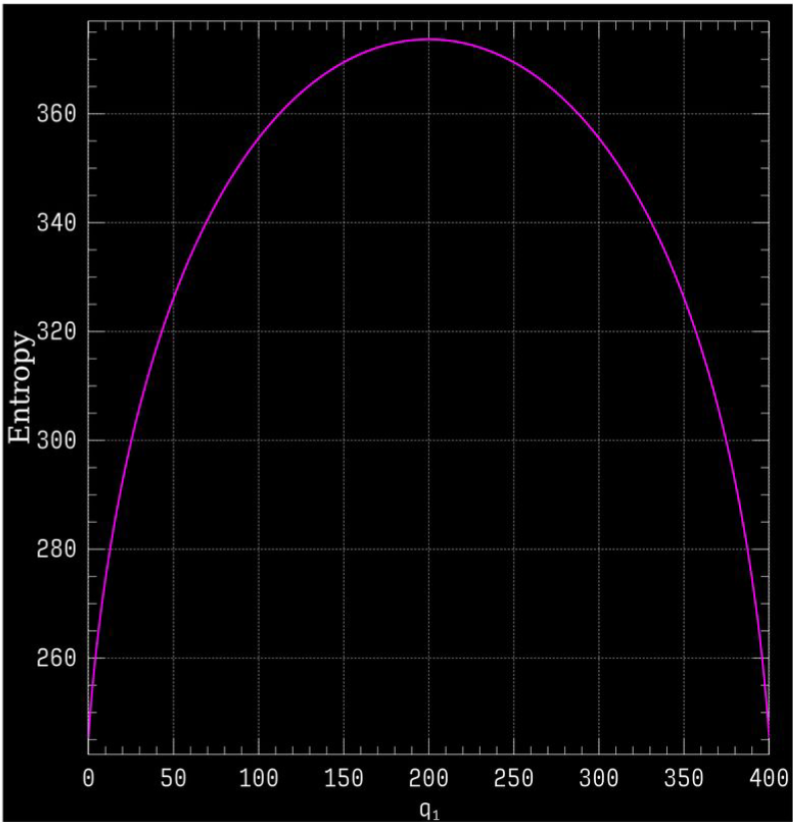
\includegraphics[width=0.8\textwidth]{entropyGraph}
            \caption{Entropy}
            \label{fig:entropyGraph}
        \end{figure}
\end{itemize}

\section{Lecture 6 -- Multiplicity of an Ideal Gas}
\begin{itemize}
    \item an ideal gas is just particles in a box
    \item recall that particles in a cubic box have energy quantized by:
        \begin{align*}
            E = \frac{h_2}{8m} \left( \frac{n_1^2+n_2^2+n_3^2}{V^{\frac{2}{3}}} \right) 
        .\end{align*}
        where $n$ is quantized (integers)
    \item multiplicity is given by
        \begin{align*}
            \Omega_N = f(m,N)V^N U^{\frac{3N}{2}}
        .\end{align*}
    \item putting two ideal gases in contact with each other:
        \begin{figure}[H]
            \centering
            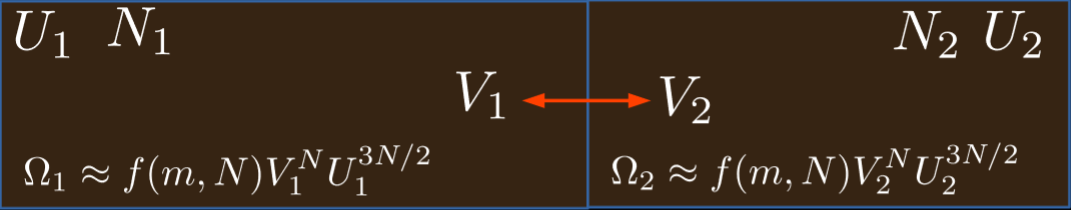
\includegraphics[width=0.8\textwidth]{multiplicityIdealGas}
            \caption{Set up for multiplicity of ideal gas.}
            \label{fig:multiplicityIdealGas}
        \end{figure}
    \item where $ N_1=N_2 \gg 1$
    \item $\Omega_{tot} = \Omega_1 \cdot \Omega_2$
    \item if we let energy $U$ flow between the two samples, then $\Omega_{tot}$ is a function of $U_1$ and $U_2$, and reaches a maximum when $U_1 = U_2 = U / 2$, i.e. when energy is evenly distributed
    \item same thing happens when you let volume  $V$ vary or number of particles  $N$ flow between the samples -- multiplicity peaks when $V_1 = V_2$, when $N_1 = N_2$
    \item in terms of entropy:
    \item entropy of a large $N$ Einstein solid: $S_1 = Nk[\ln(\frac{q_1}{N})+1]$
    \item due to how logarithms work: $S_{tot} = S_1 + S_2$
    \item we see that the entropy is higher when the energy is equally distributed between equally sized solids
    \item the entropy of an ideal gas: Sackur-Tetrode Equation
        \begin{align*}
            S = Nk \left[ \ln \left( \frac{V}{N} \left( \frac{4\pi mU}{3Nh^2} \right)^{\frac{3}{2}}  \right) + \frac{5}{2} \right] 
        .\end{align*}
        \begin{itemize}
            \item increases with $N, V, m$, and $U$
        \end{itemize}
\end{itemize}

\subsection{Entropy of Mixing}
\begin{itemize}
    \item removing the barrier between two gases
        \begin{itemize}
            \item assume that initially $ N_1 = N_2, V_1=V_2, U_1=U_2$
        \end{itemize}
    \item treat the two types of gas separately
    \item for both gases: $ N_1, U_1, m_1$ all remain constant, but $ V_1$ doubles:
        \begin{gather*}
            \Delta S_1 = \Delta S_2 = N_1 k \ln \left( \frac{V_i}{V_f} \right) =N_1k \ln (2) \\ 
            \Delta S_{tot} = 2kN\ln (2)
        .\end{gather*}
    \item what about mixing identical gases?
    \item originally, each container has an entropy of 
        \begin{align*}
            S = Nk \left[ \ln \left( \frac{V}{N} \left( \frac{4\pi mU}{3Nh^2} \right)^{\frac{3}{2}}  \right) + \frac{5}{2} \right] 
        .\end{align*}
    \item total entropy is just double that
    \item after removing the barrier, we have one system, with $N=2N_1, V = 2V_1, U = 2U_1$
    \item plugging this into the Sackur-Tetrode equation, we get
        \begin{align*}
            S = 2Nk \left[ \ln \left( \frac{V}{N} \left( \frac{4\pi mU}{3Nh^2} \right)^{\frac{3}{2}}  \right) + \frac{5}{2} \right] 
        .\end{align*}
        which is the same as what we had originally
    \item therefore $\Delta S = 0$ for identical gases
\end{itemize}



\section{Lecture 7 -- What is Temperature?}
\begin{itemize}
    \item when placed in thermal contact, the system will tend to the state with the highest entropy (i.e. $ S_1+S_2$ is maximal)
    \item but also: the system will tend to the state where the temperatures are the same
    \item peak in entropy occurs when
        \begin{gather*}
            \frac{\partial S_{tot}}{\partial q_1} = 0
        .\end{gather*}
        i.e. when 
        \begin{align*}
            \frac{\partial S_1}{\partial q_1} = \frac{\partial S_2}{q_2}
        .\end{align*}
    \item but since $U = qE_0$, peak in entropy occurs when
        \begin{align*}
            \frac{\partial S_1}{\partial U_1} = \frac{\partial S_2}{U_2}
        .\end{align*}
    \item i.e. peak occurs where you take some energy from one body and put it in the other, causing opposing changes in entropy in each body, but these changes in entropy are equal to each other and cancel out to zero (total entropy doesn't change)
        \begin{figure}[H]
            \centering
            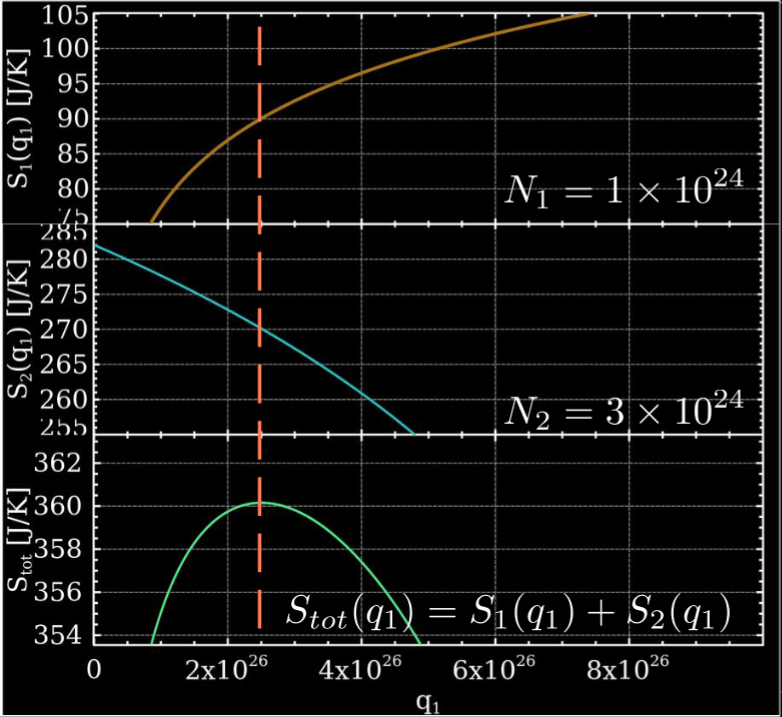
\includegraphics[width=0.8\textwidth]{entropyPeak}
            \caption{Where entropy peaks.}
            \label{fig:entropyPeak}
        \end{figure}
    \item  thermal equilibrium is when:
        \begin{enumerate}
            \item temperatures are equal
            \item entropy is maximized
        \end{enumerate}
\end{itemize}
\begin{definition}
    \textbf{Temperature (for any system)}:
    \begin{align*}
        T = \frac{\partial U}{\partial S} \quad \text{or} \quad \frac{1}{T} = \frac{\partial S}{\partial U}
    .\end{align*}
    \begin{itemize}
        \item $(T)^{-1}$ is how much entropy increases when energy is added to a system, with "everything else" held constant
        \item low temperature means $S$ increases a lot, high temperature means $S$ does not increases as much
    \end{itemize}
\end{definition}


\section{Lecture 8 -- Thermodynamic Identity}
\begin{itemize}
    \item using this model to predict heat capacity:
        \begin{enumerate}
            \item from quantum mechanics, find the multiplicity $\Omega(U,N,V,\ldots)$ 
            \item find the entropy $S = k\ln(\Omega)$ 
            \item find $T(U,N,V,\ldots) = \left( \frac{\partial S}{\partial U} \right) ^{-1}$ 
            \item solve for $U(T,N,V, \ldots)$ 
            \item find $C_V = \frac{\partial U}{\partial T}$
        \end{enumerate}
\end{itemize}

\subsection{Pressure}
\begin{itemize}
    \item consider again two systems in contact with each other, but this time we allow both volume $V$ and energy $U$ to change
    \item equilibrium occurs when $S_{max}$ 
    \item at $S_{max}$, $\frac{\partial S_1}{\partial U_1} = \frac{\partial S_2}{\partial U_2}$ and $\frac{\partial S_1}{\partial V_1} = \frac{\partial S_2}{\partial V_2}$
    \item also $T_1 = T_2$ and $P_1 = P_2$
\end{itemize}
\begin{definition}
    \textbf{Pressure (for any system)}:
    \begin{gather*}
        P = T \left( \frac{\partial S}{\partial V} \right)_{U,N}
    .\end{gather*}
    \begin{itemize}
        \item successfully reproduces the ideal gas law if we plug in the Sacker-Tetrode equation
    \end{itemize}
\end{definition}

\subsection{Chemical Potential}
\begin{itemize}
    \item now we allow volume, energy \textit{and} number $N$ to all change
    \item at equilibrium, i.e. at $S_{max}$, we have that $\frac{\partial S_1}{\partial N_1} = \frac{\partial S_2}{\partial N_2}$ 
    \item we make another definition, for chemical potential:
        \begin{definition}
            \textbf{Chemical Potential (for any system)}:
        \begin{gather*}
            \mu \equiv -T \left( \frac{\partial S}{\partial N} \right)_{U,V}
        .\end{gather*}
        \begin{itemize}
            \item at equilibrium, $\mu_1 = \mu_2$
        \end{itemize}
        \end{definition}
    \item summary of conditions of thermal equilibrium below:
\end{itemize}
\begin{figure}[H]
    \centering
    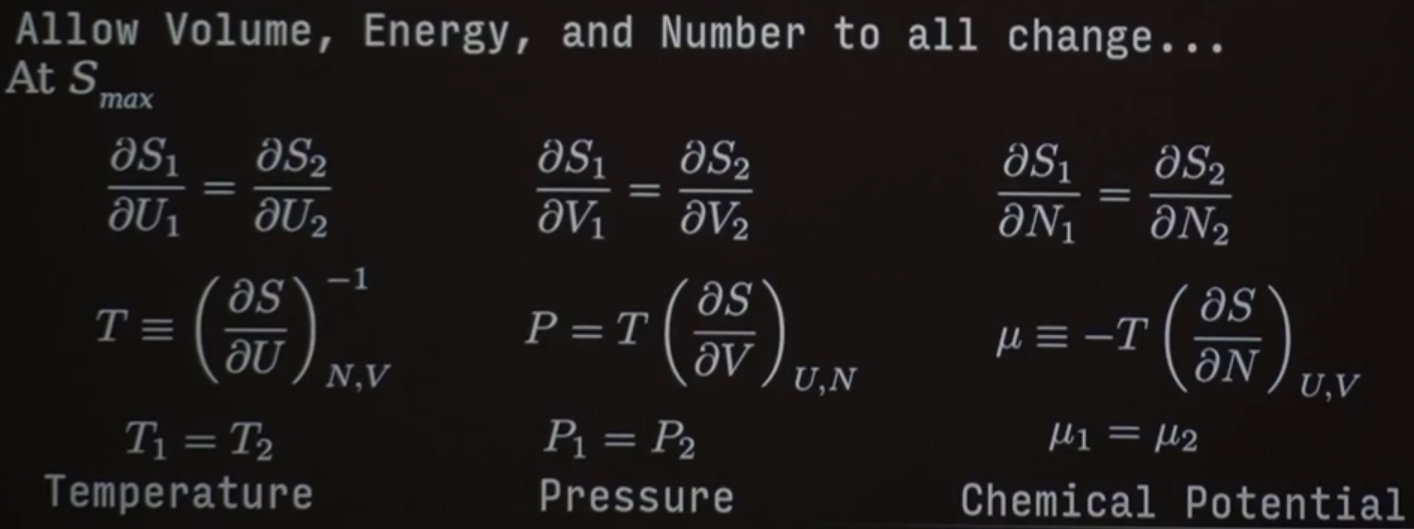
\includegraphics[width=0.8\textwidth]{thermodynamicIdentities.png}
    \caption{Summary of conditions of thermal equilibrium.}
    \label{fig:thermodynamicIdentities}
\end{figure}

\subsection{Thermodynamic Identity}
\begin{itemize}
    \item from above, we have that 
        \begin{gather*}
            dS = \left( \frac{\partial S}{\partial U}  \right)_{N,V}dU + \left( \frac{\partial S}{\partial V}  \right)_{U,N} dV + \left( \frac{\partial S}{\partial N}  \right)_{U,V} dN
        .\end{gather*}
    \item but we defined:
        \begin{gather*}
            T \equiv \left( \frac{\partial S}{\partial U}  \right)^{-1}_{N,V} \quad P = T \left( \frac{\partial S}{\partial V}  \right)_{U,N} \quad \mu \equiv -T \left( \frac{\partial S}{\partial N}  \right)_{U,V}
        .\end{gather*}
    \item so we have 
        \begin{gather*}
            dS = \frac{1}{T}dU + \frac{P}{T}dV - \frac{\mu}{T}dN
        .\end{gather*}
    \item solving for $U$ :
        \begin{theorem}
            \textbf{Thermodynamic Identity for any system}: describes behaviour of systems in thermal equilibrium
            \begin{gather*}
                dU = TdS - PdV + \mu dN
            .\end{gather*}
            \begin{itemize}
                \item this is the foundation for classical thermodynamics
            \end{itemize}
        \end{theorem}
    \item Chemcial Potential:
        \begin{itemize}
            \item keep entropy and volume constant:
                \begin{gather*}
                    \mu = \left( \frac{\partial U}{\partial N}  \right)_{S,V}
                .\end{gather*}
                \begin{itemize}
                    \item chemical potential is the amount of energy you need to add when you add a particle, in order to keep the entropy constant
                    \item since chemical potential is usually negative, you need to take away energy when you add a particle
                \end{itemize}
            \item keep energy and volume constant:
                \begin{gather*}
                    \frac{\mu}{T} = - \left( \frac{\partial S}{\partial N}  \right)_{U,V}
                .\end{gather*}
                \begin{itemize}
                    \item chemical potential (divided by temperature) is the amount the entropy changes when you add a particle while keeping energy and volume constant 
                    \item since chemical potential is usually negative, entropy increases when adding particles
                \end{itemize}
            \item keep energy and entropy constant:
                \begin{gather*}
                    \frac{\mu}{P} = \left( \frac{\partial V}{\partial N}  \right)_{U,S}
                .\end{gather*}
                \begin{itemize}
                    \item chemical potential (divided by pressure) is the amount you must change the volume when you add a particle in order to keep the energy constant
                    \item since $\mu$ is generally negative, you have to decrease the volume when adding a particle
                \end{itemize}
        \end{itemize}
    \item can apply above methods for pressure and temperature as well
\end{itemize}



\section{Lecture 9 -- Boltzmann Factors}
\begin{itemize}
    \item can we apply the thermodynamic identity to calculate cool things?
\end{itemize}
\subsection{Stellar Spectral Types}
\begin{itemize}
    \item atoms in star's atmosphere absorbs certain wavelengths of light
    \item why do hydrogen absorption lines disappear for cool stars?
        \begin{figure}[H]
            \centering
            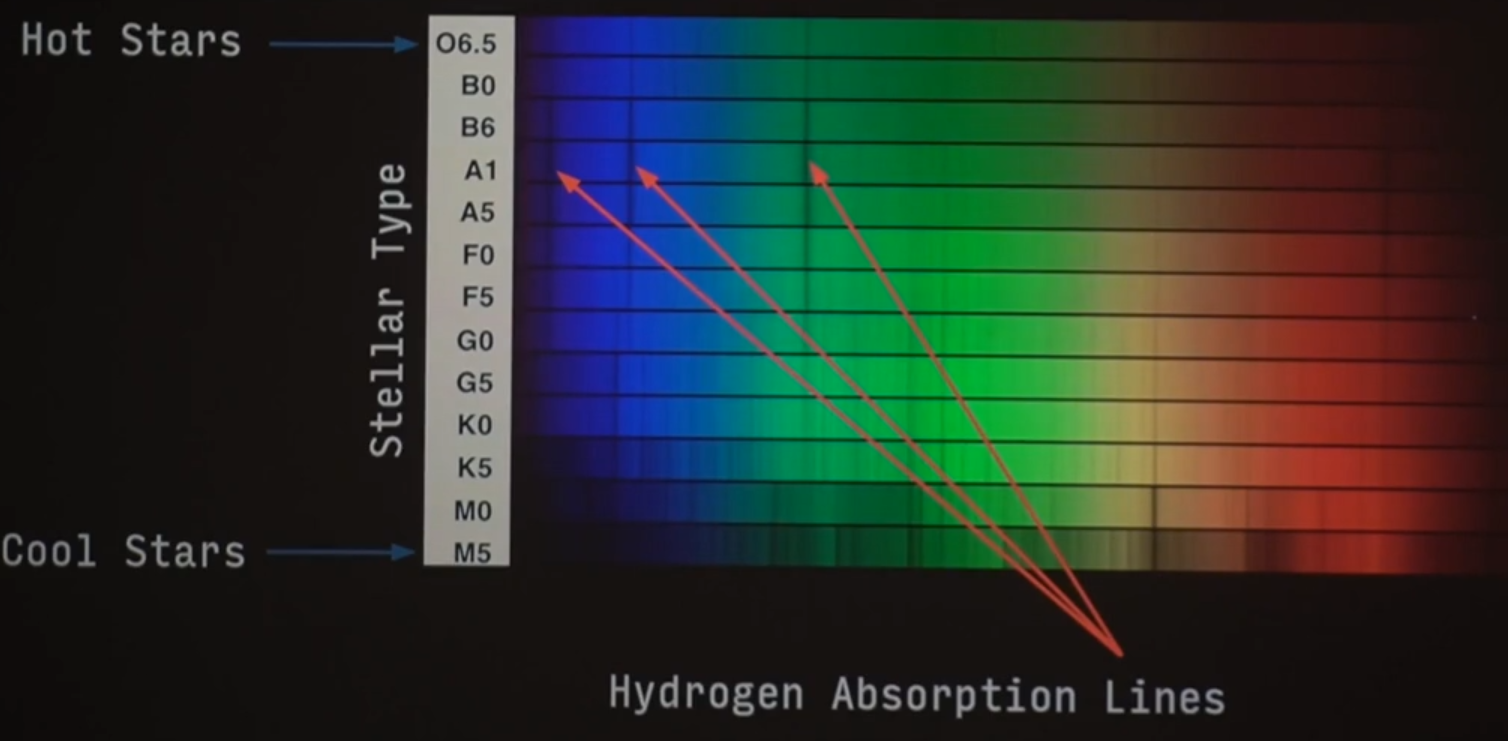
\includegraphics[width=0.8\textwidth]{starAbsorptionSpectra}
            \caption{Absorption spectra for different star temperatures.}
            \label{fig:starAbsorptionSpectra}
        \end{figure}
    \item these 3 absorption lines are from hydrogen transitions from $n=2$ to $n > 2$ 
    \item transitions from $n=1$ are in the UV 
    \item the line strength depends on the number of hydrogen atoms starting in the $n=2$ level 
    \item since cooler stars are not as hot, there are less H atoms starting in the $n=2$ level, therefore absorption lines are dimmer
    \item what is the probability that an atom will be in a particular $n=2$ mode compared to a particular $n=1$ mode? (call these $s_1$ and $s_2$)
        \begin{gather*}
            \frac{P(s_2)}{P(s_1)} = \frac{\Omega_R(s_2)}{\Omega_R(s_1)}
        .\end{gather*}
    \item $\Omega_R$ is the multiplicity of the Sun's atmosphere (the reservoir) when the atom (the subsystem) is in state 2
    \item after some math, subbing in $S = k\ln(\Omega)$, and we only allow energy to flow ($dN=0, dV=0$), and using the thermodynamic identity, we obtain:
        \begin{gather*}
            \frac{P(s_2)}{P(s_1)} = \frac{e^{-E(s_2) / kT}}{e^{-E(s_1) / kT}}
        .\end{gather*}
        \begin{itemize}
            \item where  $E(s)$ is the energy level of the subsystem in microstate $s_2$ 
            \item $T$ is temperature of reservoir 
            \item \textbf{Boltzmann Factor}: $e^{-E(s) / kT}$
        \end{itemize}
    \item the probability of a given microstate $s_i$ of a subsystem in equilibrium with a reservoir at temperature $T$ :
        \begin{gather*}
            P(s_i) = \frac{1}{Z} e^{-E(s_i) / kT}
        .\end{gather*}
    \item $Z$ is the \textbf{Partition Function} -- the sum of the Boltzmann Factors of all possible microstates that the subsystem could ever be in: 
        \begin{gather*}
            Z = \sum_{s} e^{-E(s) / kT}
        .\end{gather*}
        \begin{figure}[H]
            \centering
            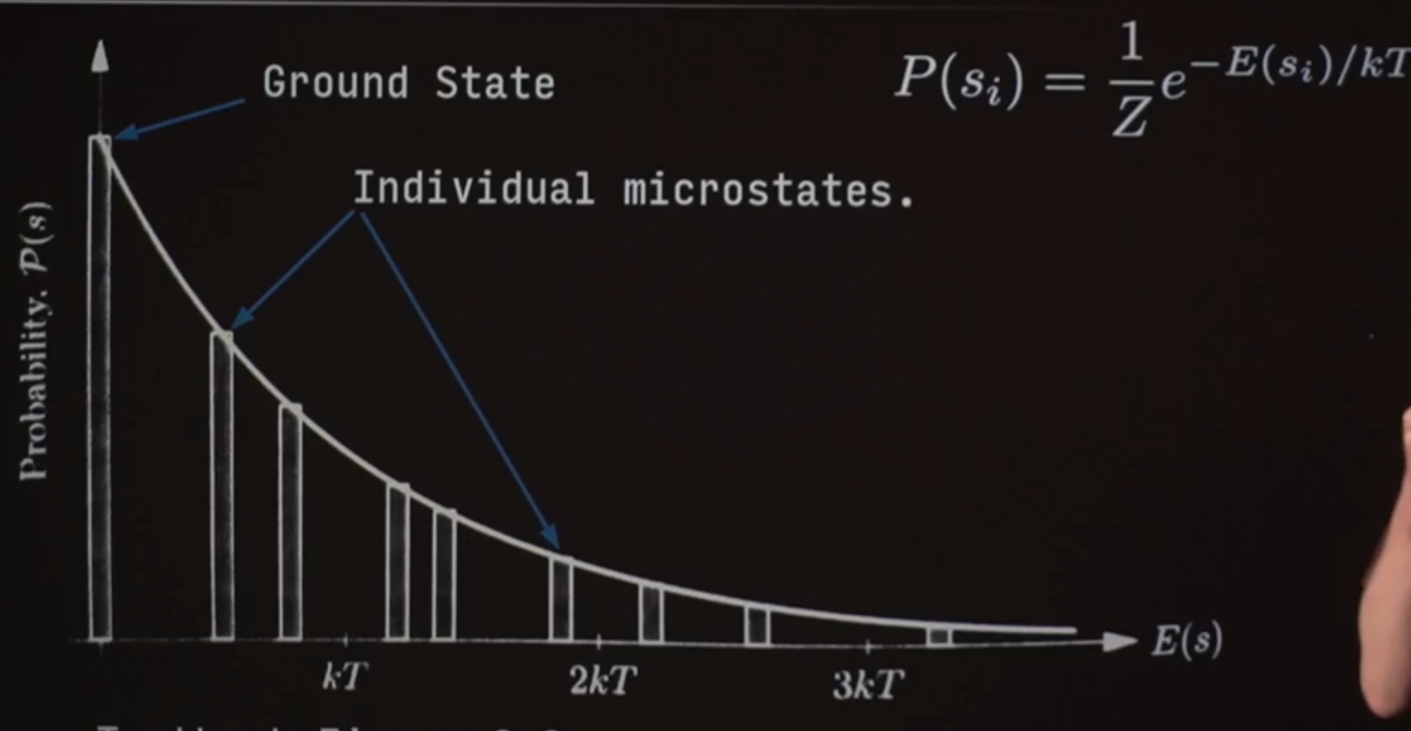
\includegraphics[width=0.8\textwidth]{partitionFunction}
            \caption{Plotting probability of being in a certain state. Increasing energy of subsystem means taking energy away from reservoir, which decreases the multiplicity of the reservoir, which decreases the entropy, therefore making it less likely (lower probability).}
            \label{fig:partitionFunction}
        \end{figure}
    \item there may be multiple microstates with the same energy, but each has the same probability
    \item multiplicity of $n=1$ is 1, of $n=2$ is 4, then
        \begin{gather*}
            \frac{P(n=2)}{P(n=1)} = 4e^{-\Delta E / kT}
        .\end{gather*}
        \begin{figure}[H]
            \centering
            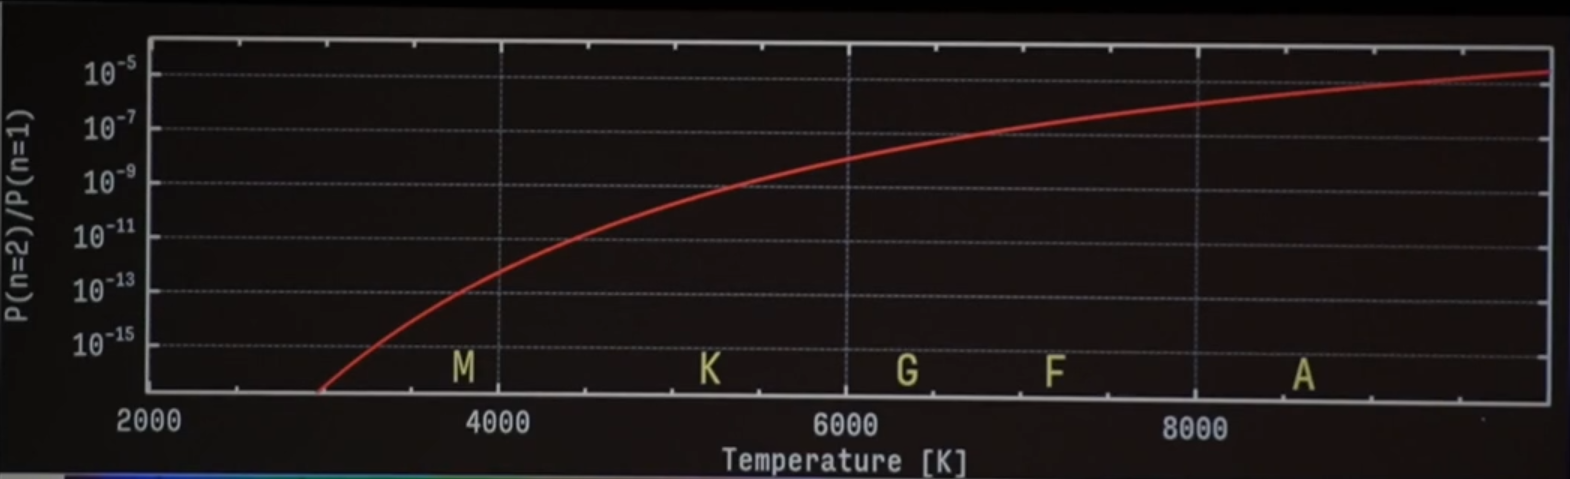
\includegraphics[width=0.8\textwidth]{stateProbability}
            \caption{Plot of probability of $n=2$ state vs $n=1$ state (probability ratio).}
            \label{fig:stateProbability}
        \end{figure}
    \item at low temperatures, the $n=2$ level is insufficiently populated for hydrogen absorption lines to appear
    \item point is, this equation is crazy:
        \begin{gather*}
            \frac{P(s_2)}{P(s_1)} = \frac{e^{-E(s_2) / kT}}{e^{-E(s_1) / kT}}
        .\end{gather*}
    \item basically, if you measure the temperature of something, you can predict the probability that a subsystem will be at a particular energy level, which is cool and a lot can be done with this
    \item \textbf{note: this is only applicable for fixed $N$ and $V$}
\end{itemize}



\section{Lecture 10 -- Average Values}
\begin{itemize}
    \item consider some parameter $X(s)$ that is a function only of the quantum-mechanical mode the subsystem is in (e.g. energy, angular momentum, quantum number, velocity, etc.), then its \textbf{average value} is 
        \begin{gather*}
            \overline{X} = \sum_{s} P(s)X(s) = \frac{1}{Z} \sum_{s} X(s) e^{-E(s) \beta}
        .\end{gather*}
        where $\beta \equiv 1 / kT$
    \item in particular, \textbf{average energy} $\overline{E}$ is 
        \begin{gather*}
            \overline{E} = \frac{1}{Z} \sum_{s} E(s)e^{-E(s)\beta} \\ 
            \text{some math\ldots} \\ 
            = -\frac{1}{Z} \frac{\partial Z}{\partial \beta} 
        .\end{gather*}
    \item this can be used to predict a lot of complex behaviours (e.g. heat capacity) very accurately
\end{itemize}

\subsection{Generalized Equipartition Theorem}
\begin{itemize}
    \item consider a quantum system where the energy levels are given by $E_n = Cn^m$ where $n=0,1,2,\ldots,\infty$, and no degeneracy 
    \item in this subsystem, keep the number of particles and volume fixed, then 
        \begin{gather*}
            \overline{E} = -\frac{1}{Z} \frac{\partial Z}{\partial \beta} = \; \text{a lot of math\ldots} \; = \frac{kT}{m}
        .\end{gather*}
\end{itemize}
\begin{theorem}
    \textbf{Equipartition Theorem (no degeneracy)}: when $E_n = Cn^m$ with  $n=0,1,2,\ldots,\infty$, no degeneracy, and $C / kT \ll 1$, then average energy $\overline{E}$ is given by 
    \begin{gather*}
        \overline{E} = \frac{kT}{m}
    .\end{gather*}
\end{theorem}
\begin{itemize}
    \item now consider the same system, except there is degeneracy, and the number of modes is given by $N_s = Dn^a$
\end{itemize}
\begin{theorem}
    \textbf{Equipartition Theorem (with degeneracy)}: when $E_n = Cn^b$ with  $n=0,1,2,\ldots,\infty$, $N_s = Dn^a$, and $C / kT \ll 1$, then average energy $\overline{E}$ is given by 
    \begin{gather*}
        \overline{E} = \frac{(a+1)kT}{b}
    .\end{gather*}
\end{theorem}




\section{Lecture 11 -- Maxwell Speed Distribution}
\begin{itemize}
    \item can we use Boltzmann factors to calculate the speed distribution of particles in an ideal gas?
    \item should be able to -- Boltzmann factors can be used to calculate probability of finding a particle in a certain quantum mode
    \item we want to calculate $D(v)$, the probability density for the speed
    \item the molecule has \textit{some} speed, so: 
        \begin{gather*}
            \int_{0}^{\infty} D(v) dv = 1
        .\end{gather*}
    \item we also know that 
        \begin{gather*}
            D(v) \propto \text{(probability of being in a state with speed $v$)} \times \text{(density of states with speed $v$)} \\ 
            D(v) \propto e^{-E(v) / kT} \times N(v)
        \end{gather*}
    \item and since $N(v) \propto v^2$
         \begin{gather*}
            D(v) \propto e^{-mv^2 / 2kT} \times v^2 \\ 
            D(v) = Cv^2 e^{-mv^2 / 2kT}
        .\end{gather*}
        where $C$ is some constant
    \item subbing this into the integral and solving for $C$, we obtain this result for $D(v)$: 
        \begin{gather*}
            D(v) = 4\pi \left( \frac{m}{2\pi kT} \right)^{3 / 2} v^2 e^{-mv^2 / 2kT}
        .\end{gather*}
        \begin{figure}[H]
            \centering
            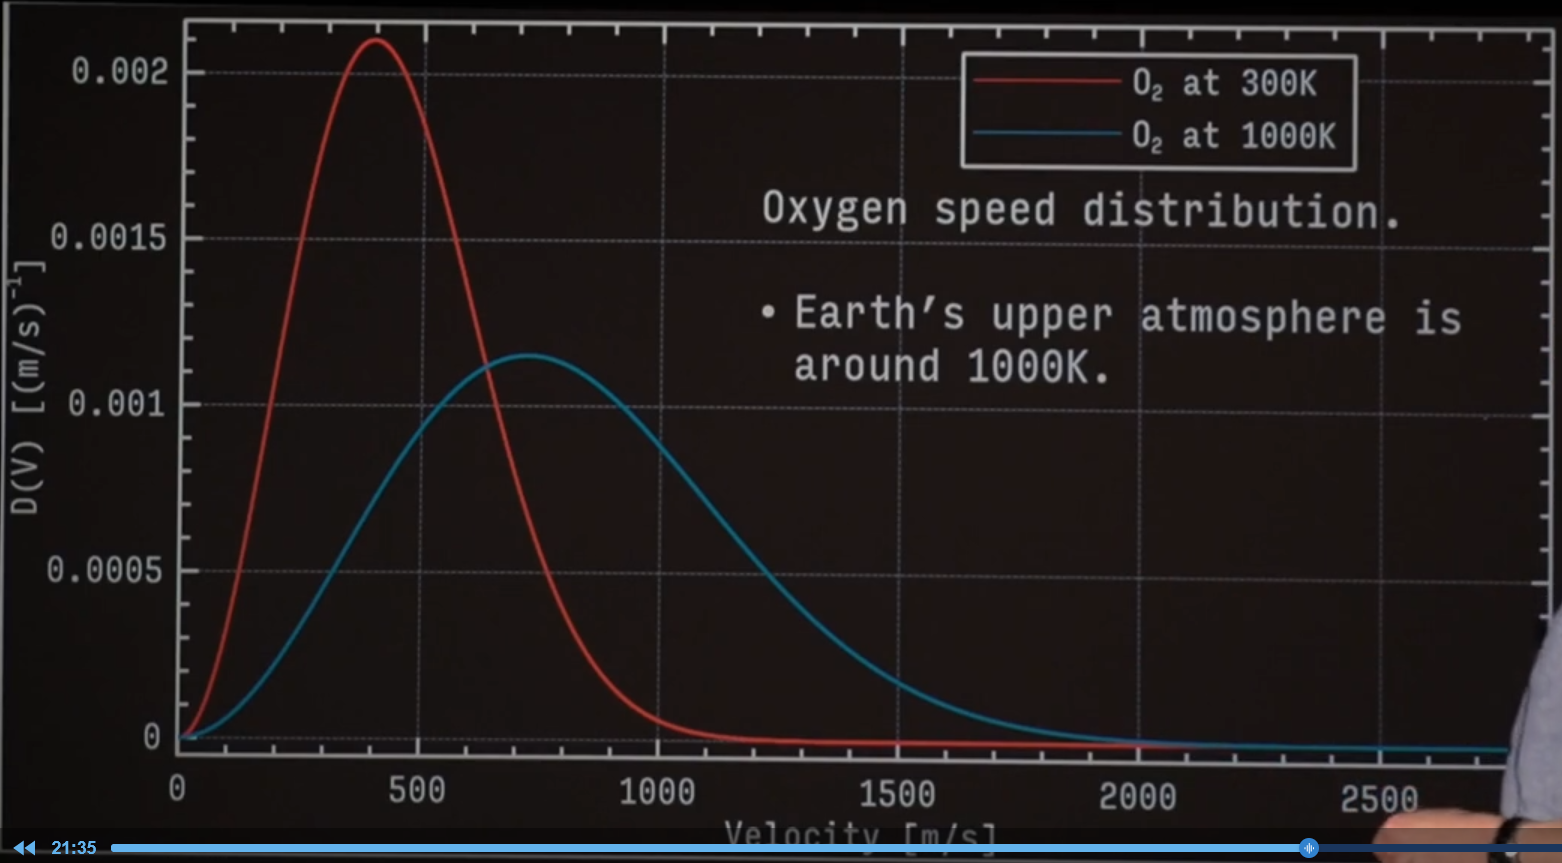
\includegraphics[width=0.8\textwidth]{speedDistribution}
            \caption{Maxwell speed distribution for oxygen at different temperatures.}
            \label{fig:speedDistribution}
        \end{figure}
    \item every planet has an escape velocity
    \item upper atmosphere of Earth is around 1000K -- extremely tiny fraction of oxygen at this temperature is actually fast enough to escape compared to how much oxygen is on Earth
    \item helium at 1000K is faster and therefore our atmosphere has less helium
    \item cool thing: we can calculate atmospheric composition from Boltzmann statistics
\end{itemize}




\section{Lecture 12 -- Free Energy}
Recap:
\begin{itemize}
    \item \textbf{Boltzmann Factor:} the probability that a subsystem is in a particular quantum mode $s$ with energy $E$ is proportional to
        \begin{gather*}
            e^{-E(s) / kT}
        .\end{gather*}
        \begin{itemize}
            \item a subsystem where every possible quantum mode can be enumerated (e.g. molecules in a box) and we can list their degeneracies
            \item subsystem is in equilibrium with some bath at temperature $T$
        \end{itemize}
    \item the proportionality constant is $1 / Z$ where $Z$ is the \textbf{Partition Function} (sum of all Boltzmann factors):
        \begin{gather*}
            Z = \sum_{s} e^{-E(s) / kT}
        .\end{gather*}
    \item partition function can be used to calculate the average value of some quantity, notably the energy:
        \begin{gather*}
            \overline{E} = \frac{1}{Z} \sum_{s} E(s) e^{-E(s) \beta} = -\frac{1}{Z} \frac{\partial Z}{\partial \beta} \\ 
            \beta \equiv \frac{1}{kT}
        .\end{gather*}
    \item the partition function can do a lot more\ldots
\end{itemize}

\subsection{Partition Function for Combined Systems}
\begin{itemize}
    \item Distinguishable subsystems: imagine $s_1$ and $s_2$ represent the quantum states of two distinguishable non-interacting subsystems
        \begin{itemize}
            \item for example: $s_1$ is the rotational mode and $s_2$ is the translational mode of a particle 
            \item another example: $s_1$ is translational mode for an O$_2$ molecule in a box and $s_2$ is the translational mode for an N$_2$ molecule the same box
        \end{itemize}
    \item then 
        \begin{gather*}
            Z = Z_1Z_2
        .\end{gather*}
    \item more generally:
        \begin{gather*}
            Z_{tot} = \prod_{i} Z_i 
        .\end{gather*}
    \item but what if they are indistinguishable?
    \item conisder two indistinguishable subsystems (eg. two He atoms in the same box):
    \item if we say that $Z = Z^2$ then we will have overcounted by a factor of $N!$ since for example $s_1=4, s_2 = 1$ represents the exact same state as $s_1 = 1, s_2=4$ 
    \item i.e. for indistinguishable subsystems:
        \begin{gather*}
            Z_{tot} = \frac{Z_1^N}{N!}
        .\end{gather*}
\end{itemize}

\subsection{Helmholtz Free Energy}
\begin{definition}
    \textbf{Helmholtz Free Energy}:
    \begin{gather*}
        F \equiv U-TS
    .\end{gather*}
    But also:
    \begin{gather*}
        F = -kT \ln Z
    .\end{gather*}
\end{definition}
\begin{itemize}
    \item $F$ is a function of the partition function $Z$ which can be calculated for quantum systems, which means that we can also determine $F$ for quantum systems
    \item also, since $F \equiv U-TS$, we can use it to calculate $S$, $P$, and $\mu$, which is huge:
        \begin{gather*}
            S = -\left( \frac{\partial F}{\partial T}  \right)_{V,N} \quad P = - \left( \frac{\partial F}{\partial V}  \right)_{T,N} \quad \mu = - \left( \frac{\partial F}{\partial N}  \right)_{T,V}
        .\end{gather*}
    \item \textbf{Steps to knowing stuff}:
        \begin{enumerate}
            \item calculate $Z$
            \item from $Z$, calculate $U, C_V, F, S, P, \mu$
        \end{enumerate}
\end{itemize}

\subsection{Ideal Gases (again)}
\begin{itemize}
    \item first we calculate $Z$ for 1 particle in a cubic box of length $L$ 
    \item can be separated into 3 distinguishable subsystems: translational, diatomic rotational, and diatomic vibrational modes ($Z_{tr}, Z_{rot}, Z_{vib}$)
    \item since they are distinguishable:
        \begin{gather*}
            Z_1 = Z_{tr}Z_{rot}Z_{vib} = Z_{tr}Z_{int}
        .\end{gather*}
    \item now for $N$ molecules, since they are indistinguishable:
        \begin{gather*}
            Z_N = \frac{Z_{tr}^N Z_{int}^N}{N!}
        .\end{gather*}
    \item we know that 
        \begin{gather*}
            U = -\frac{1}{Z} \frac{\partial Z}{\partial \beta} = - \frac{\partial \ln Z}{\partial \beta} 
        .\end{gather*}
    \item we can use this to calculate a bunch of things: from this we get 
        \begin{gather*}
            C_V = \frac{3}{2}Nk + \frac{\partial U_{int}}{\partial T} \\ 
            P = \frac{kTN}{V} \quad \text{(ideal gas law)}
        .\end{gather*}
    \item this is incredibly powerful -- if we can enumerate the quantum modes for a subsystem, then we can calculate the partition function for it, and from this we can calculate a huge number of things
    \item note: this is assuming that the number of particles and volume stays constant
    \item so far, we've only looked at the partition function where energy can change but number of particles $N$ is constant 
    \item next: we look at the grand partition function where both energy and $N$ can change
\end{itemize}





\section{Lecture 13 -- Gibbs Factors}
\begin{itemize}
    \item when we let the number of particles $N$ vary, we call it \textbf{Gibbs Factors} instead of Boltzmann factors
    \item but volume is still kept constant
    \item then we get 
        \begin{gather*}
            \frac{P(s_2)}{P(s_1)} = \frac{e^{-[E(s_2) - \mu N(s_2)] / kT}}{e^{-[E(s_1) - \mu N(s_1)] / kT}}
        .\end{gather*}
    \item where the \textbf{Gibbs Factor} is 
        \begin{gather*}
            e^{-[E(s) - \mu N(s)] / kT}
        .\end{gather*}
        \begin{itemize}
            \item $E(s)$ is the energy level of the subsystem in microstate state $s$
            \item $N$ is the number of particles in the subsystem in microstate state $s$
        \end{itemize}
    \item then the probability of a given microstate of a subsystem in equilibrium with a reservoir at temperature $T$ is: 
        \begin{gather*}
            P(s) = \frac{1}{\mathcal{Z}} e^{-[E(s) - \mu N(s)] / kT}
        .\end{gather*}
        where $\mathcal{Z}$ is the \textbf{Grand Partition Function}: 
        \begin{gather*}
            \mathcal{Z} = \sum_{s} e^{-[E(s) - \mu N(s)] / kT}
        .\end{gather*}
    \item pretty much same as Boltzmann stuff except now we keep track of entropy change when number of particles change -- therefore we have a $\mu N$ term
\end{itemize}




\section{Lecture 14 -- Degenerate Fermi Gas}
\begin{itemize}
    \item \textbf{Bosons vs Fermions}:
        \begin{itemize}
            \item Fermions: only one particle allowed in a given quantum state (electrons, protons, neutrons, anything with spin half)
            \item Bosons: no limit to number of particles allowed in a given quantum state (photons, pions, etc.)
        \end{itemize}
    \item previously we said that for indistinguishable subsystems 
        \begin{gather*}
            Z_{tot} = \frac{Z_1^N}{N!}
        .\end{gather*}
        \textbf{but this is only true when $Z\gg N$} 
    \item since bosons can occupy the same quantum state, the number of allowed states will be greater than fermions, but this difference in number of allowed states becomes negligible when the total number of states is much larger than the number of particles
    \item how to deal with fermions when $Z \gg N$ is not true and whether or not the particles are bosons or fermions matters?
    \item instead of thinking about what quantum mode a particle is in, think about how many particles are in a certain quantum mode with $E = \epsilon$
    \item for fermions: $N = 0$ or $N = 1$ 
    \item so then the Gibbs Factors are:
        \begin{itemize}
            \item for empty state ($N=0, E=0$): 1 
            \item for full state ($N=1, E=\epsilon$): $e^{-[\epsilon-\mu] / kT}$
        \end{itemize}
    \item grand partition function is sum of these factors: $\mathcal{Z} = 1 + e^{-[\epsilon-\mu] / kT}$
    \item and the probability that there will be 1 particle in this mode is 
        \begin{gather*}
            P(1) = \frac{1}{\mathcal{Z}}e^{-[\epsilon-\mu] / kT}
        .\end{gather*}
    \item then if we want to find the average number of particles in this quantum mode: 
        \begin{gather*}
            \overline{n} = \sum_{n} P(n) = (0 \cdot P(0)) + (1 \cdot P(1))
        .\end{gather*}
    \item simplifying, this gives us the average number of particles in the quantum mode (some value between 0 and 1):
        \begin{gather*}
            \overline{n}_{FD} = \frac{1}{e^{(\epsilon-\mu) / kT} + 1}
        .\end{gather*}
    \item plot of this function: the \textbf{Fermi Dirac Distribution Function} 
        \begin{figure}[H]
            \centering
            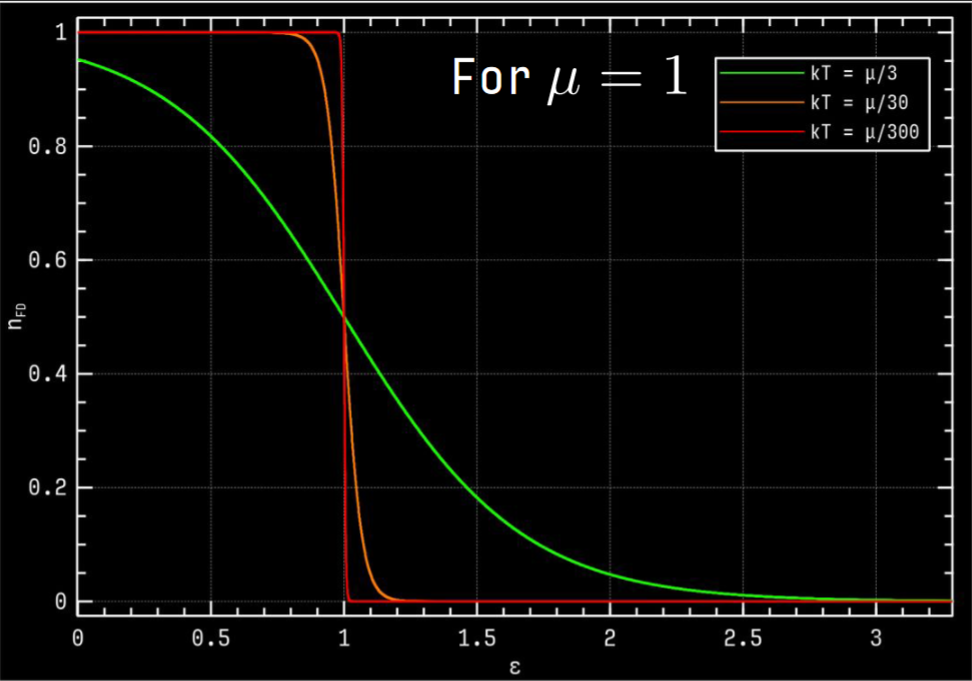
\includegraphics[width=0.8\textwidth]{fermiDirac}
            \caption{The Fermi Dirac Distribution.}
            \label{fig:fermiDirac}
        \end{figure}
    \item we see that at very low temperatures, there will pretty much always be a particle occupying a low energy state (below $\epsilon = \mu = \epsilon_F$) and the chance of a particle occupying an energy state higher than that is zero
    \item particles try to bunch up in low energy states
    \item but at higher temperatures, particles start to move to higher energy states and it begins to look more like a Boltzmann distribution
\end{itemize}

\subsection{Neutron Stars}
\begin{itemize}
    \item consider a gravitationally bound object made only of neutrons 
        \begin{itemize}
            \item gravity is holding it together 
            \item neutrons are uncharged so no electrostatic repulsion 
            \item neutrons are fermions 
        \end{itemize}
    \item how small does it get? Why doesn't it contract to zero size?
    \item after a bunch of math we find that:
        \begin{itemize}
            \item pressure is given by 
                \begin{gather*}
                    P = \frac{h^2}{20m} \left( \frac{3}{\pi} \right)^{2 / 3} \left( \frac{N}{V} \right)^{5 / 3}
                .\end{gather*}
            \item notice that this is \textbf{not} the ideal gas law 
                \begin{itemize}
                    \item it is a faster function of $V$ and $N$ and it is independent of $T$ 
                    \item the fermi energy $\epsilon_F$ of neutron stars are so high that even very hot neutron stars are essentially at zero temperature (hence independence of $T$) and the neutrons will try to bunch up in the lowest quantum mode
                    \item it is called the \textbf{Degeneracy Pressure} since it is only caused by the fact that neutrons are fermions (can't occupy same quantum mode) and it has nothing to do with electrostatic repulsion
                \end{itemize}
            \item we also find: radius decreases with neutron star mass
            \item maximum velocity of the neutrons increases with the mass of the star, and as $v_{max}$ approaches the speed of light, the neutron star becomes unstable since the degeneracy pressure can no longer hold it up and collapses into a black hole
            \item neutron stars are typically have a radius of 11 km -- they have more mass than the sun but are only around the size of a city
        \end{itemize}
    \item point is: it's crazy how we can calculate so much about neutron stars only from statistics
\end{itemize}




\section{Lecture 15 -- Blackbody Radiation}
\begin{itemize}
    \item previously we looked at how to deal with fermions when $Z\gg N$ is not true
    \item now: how to deal with bosons when $Z \gg N$ is not true?
    \item again we think about the number of particles in a particular quantum mode with $E = n\epsilon$ and $N = n$
    \item for bosons,  $n$ goes from 0 to $\infty$
    \item then, following the same logic that we did for fermions:
        \begin{gather*}
            \text{Gibbs Factors:} \quad e^{-n(\epsilon-\mu) / kT} \\ 
            P(n) = \frac{1}{\mathcal{Z}}e^{-n(\epsilon-\mu) / kT} \\
            \mathcal{Z} = \sum_{n=0}^{\infty} e^{-n(\epsilon-\mu) / kT} = \frac{1}{1-e^{-(\epsilon-\mu) / kT}} \\
            \overline{n} = \sum_{n=0}^{\infty} nP(n) = \frac{1}{e^{(\epsilon-\mu) / kT} - 1}
        .\end{gather*}
        where the average number of particles occupying a particular quantum mode is given by the \textbf{Bose-Einstein Distribution Function}:
        \begin{gather*}
            \overline{n}_{BE} = \frac{1}{e^{(\epsilon-\mu) / kT} - 1}
        .\end{gather*}
        \begin{figure}[H]
            \centering
            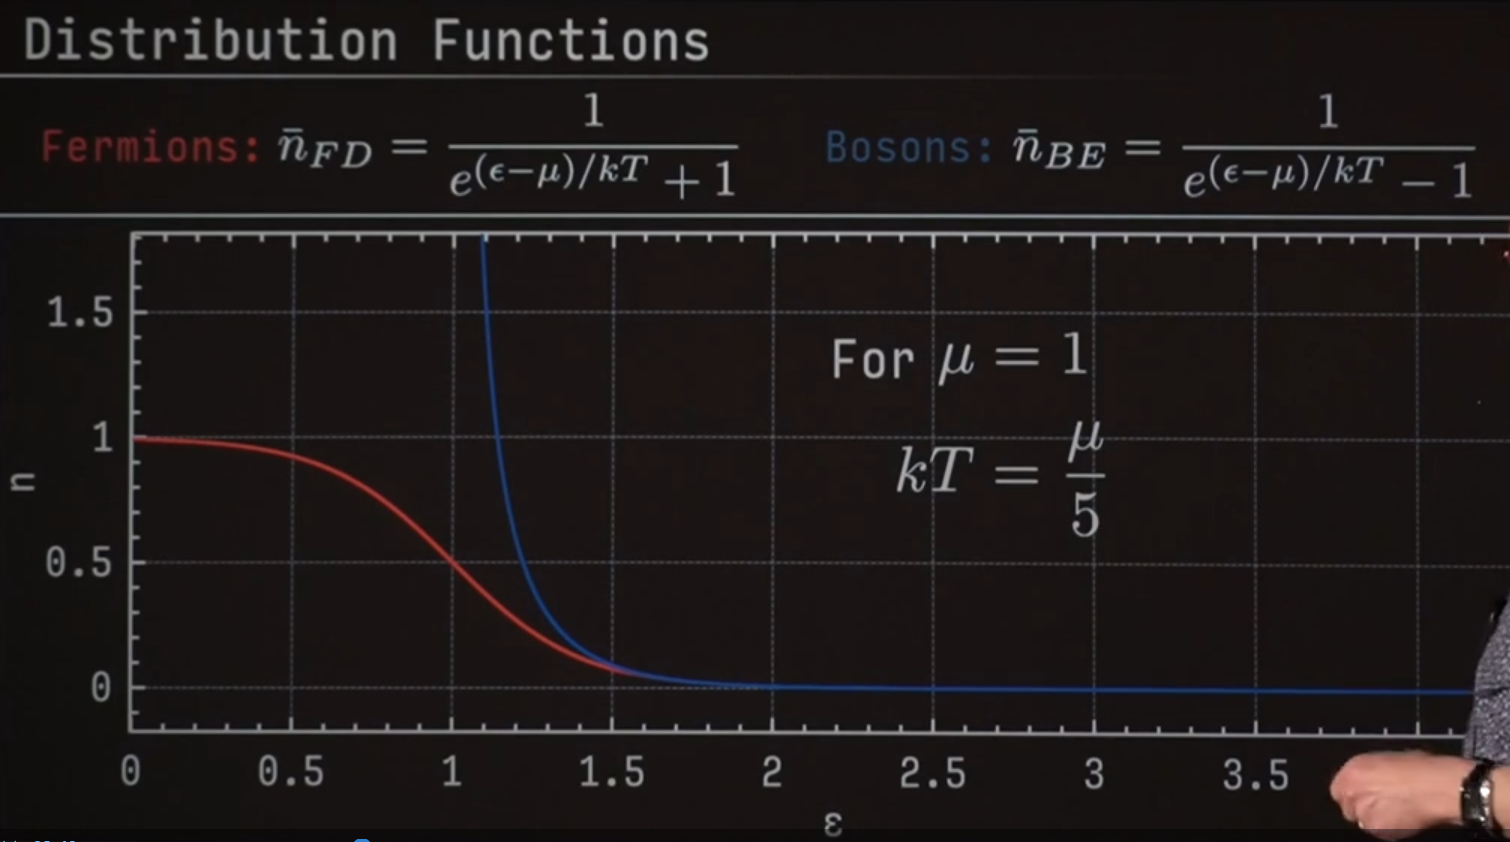
\includegraphics[width=0.8\textwidth]{boseEinstein}
            \caption{Bose-Einstein Distribution Function.}
            \label{fig:boseEinstein}
        \end{figure}
    \item we can see that instead of reaching a maximum of 1, the number of particles in a quantum mode goes to infinity as the energy decreases since all particles want and are able to occupy the lowest state
\end{itemize}

\subsection{Blackbodies}
\begin{itemize}
    \item all incident light is absorbed (none reflected)
    \item we care because we observe that hot things glow -- why? how?
    \item can model a blackbody as a box with a tiny hole (hole is black)
    \item we want to find the energy of photons in the box 
    \item we can first ignore the hole and calculate energy density in the box, then later put the hole back and look at what leaks out 
    \item our strategy:
        \begin{enumerate}
            \item Find the energy levels $E_s$ of all photons that could be in the box (listing all quantum modes) 
            \item Find the occupancy $\overline{n}_s$ for these energy levels (find how many photons are in each quantum mode)
            \item $U = \sum_{s} E_s \overline{n}_s$ : add it all up
        \end{enumerate}
\end{itemize}
\subsubsection*{Step 1: Find the energy levels of photons in box}
\begin{itemize}
    \item there are standing waves in the box 
    \item energy is given by 
        \begin{gather*}
            E = |\bm{p}|c = \frac{jhc}{2L} 
        \end{gather*}
        where
        \begin{gather*}
            j = \sqrt{j_x^2 + j_y^2 + j_z^2} 
        .\end{gather*}
\end{itemize}
\subsubsection*{Step 2: Find $\overline{n}$ per mode}
\begin{itemize}
    \item on average, how many photons are in each mode? i.e. what is the occupancy?
    \item photons are bosons so $\overline{n}$ is given by the formula for  $\overline{n}_{BE}$
    \item we know $\epsilon$, but what is $\mu$ for a photon?
    \item $\mu$ for a photon is given by 
        \begin{gather*}
            \mu_{\text{photon}} = -T \left( \frac{\partial S}{\partial N} \right)_{U,V}
        .\end{gather*}
        \begin{itemize}
            \item $T$ is the temperature of the reservoir (walls of the box)
            \item $\partial S$ is change in entropy of the reservoir 
        \end{itemize}
    \item recall: photons are not conserved, so if you keep the reservoir's energy constant, the reservoir's entropy doesn't change at all when you add a photon to the subsystem (reservoir = walls of the box), therefore: 
        \begin{gather*}
            \mu_{photon} = 0
        .\end{gather*}
        \begin{itemize}
            \item doesn't cost anything in terms of entropy to create another photon -- they're "free"
        \end{itemize}
    \item now we know $\mu_{photon}$, so the occupancy for a certain wavelength is:
        \begin{gather*}
            \overline{n}_{\lambda} = \frac{1}{e^{\epsilon / kT} - 1}
        .\end{gather*}
        where $\epsilon$ is the energy $E$ of the wavelength we found in Step 1
\end{itemize}
\subsubsection*{Step 3: Find total energy, $U$}
\begin{itemize}
    \item we use $U = \sum_{s} E\overline{n}$
    \item we can assume that size of the box and temperature is large, so we can replace sums with integrals
        \begin{gather*}
            U = \int_{0}^{\infty} \frac{8\pi L^3 \epsilon^3}{(hc)^3(e^{\epsilon / kT} - 1)} d \epsilon 
        .\end{gather*}
    \item note that $V = L^3$, so the energy density of photons in an enclosed box of uniform wall temperature $T$ is 
        \begin{gather*}
            \frac{U}{V} = \int_{0}^{\infty} \frac{8\pi \epsilon^3}{(hc)^3(e^{\epsilon / kT} - 1)} d \epsilon 
        .\end{gather*}
    \item then the energy density per energy band of photons is
        \begin{gather*}
            u = \frac{d(U / V)}{d \epsilon} = \frac{8\pi}{(hc)^3}\frac{\epsilon^3}{e^{\epsilon / kT} - 1}
        .\end{gather*}
    \item plotting this: 
        \begin{figure}[H]
            \centering
            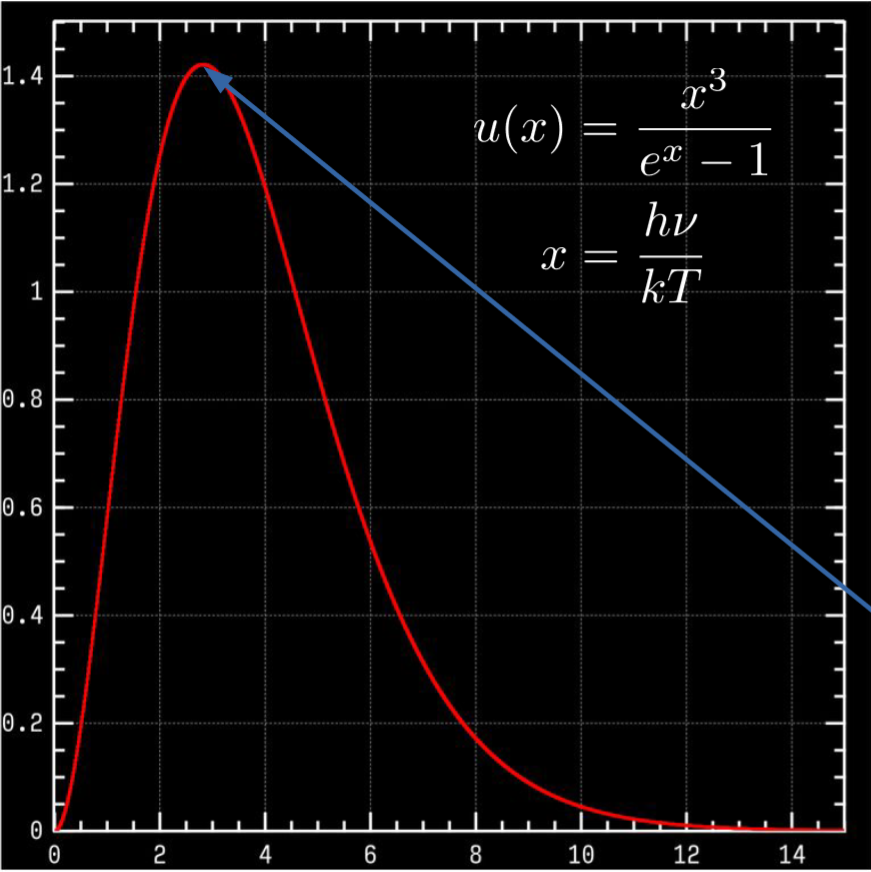
\includegraphics[width=0.6\textwidth]{blackbodyEnergy}
            \caption{Plot of $u$.}
            \label{fig:blackbodyEnergy}
        \end{figure}
    \item frequency of light inside the box takes that shape and peaks at $\nu_{peak} \approx 2.82kT / h$
    \item so as $T$ increases the curve shift right, as $T$ decreases the curve shifts left
    \item evaluating the integral for the total energy density, we get 
        \begin{gather*}
            \frac{U}{V} = \frac{8\pi^5 k^4}{15(hc)^3}T^4
        .\end{gather*}
\end{itemize}

\subsubsection*{Letting Light Out}
\begin{itemize}
    \item now we poke a hole in the box and see how much energy escapes 
        \begin{figure}[h]
            \centering
            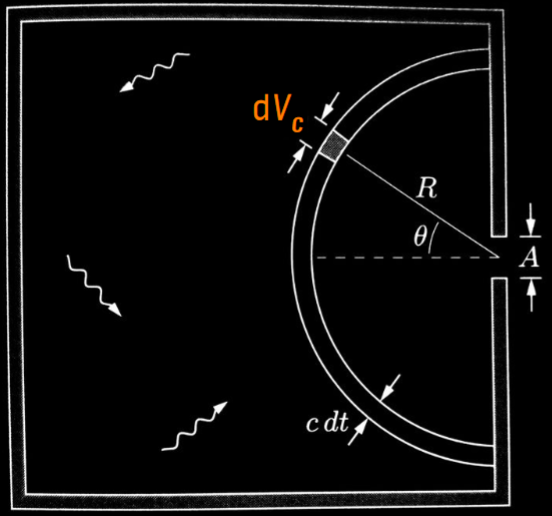
\includegraphics[width=0.6\textwidth]{blackbodyHole}
            \caption{Setup for huge amounts of math that is skipped in these notes lol.}
            \label{fig:blackbodyHole}
        \end{figure}
    \item after a lot of math, we find that the amount of energy that escapes in time $dt$ is 
        \begin{gather*}
            E_{esc} = \frac{A}{4} \frac{U}{V} cdt 
        .\end{gather*}
    \item then power is 
        \begin{gather*}
            P = \frac{E_{esc}}{dt} = c \frac{A}{4} \frac{U}{V}
        .\end{gather*}
    \item and so the power that escapes per unit area of the hole is given by: 
        \begin{gather*}
            \frac{P}{A} = \frac{c}{4} \frac{U}{V} = \frac{2\pi^5 k^4}{15h^3c^2} T^4 = \sigma T^4
        .\end{gather*}
    \item this is true for any black object (not just a hole in a box)
    \item this doesn't account for reflective things though -- they behave differently
\end{itemize}

\subsection{Cool Applications in Astrophysics}
\begin{itemize}
    \item consider the universe 
        \begin{figure}[h]
            \centering
            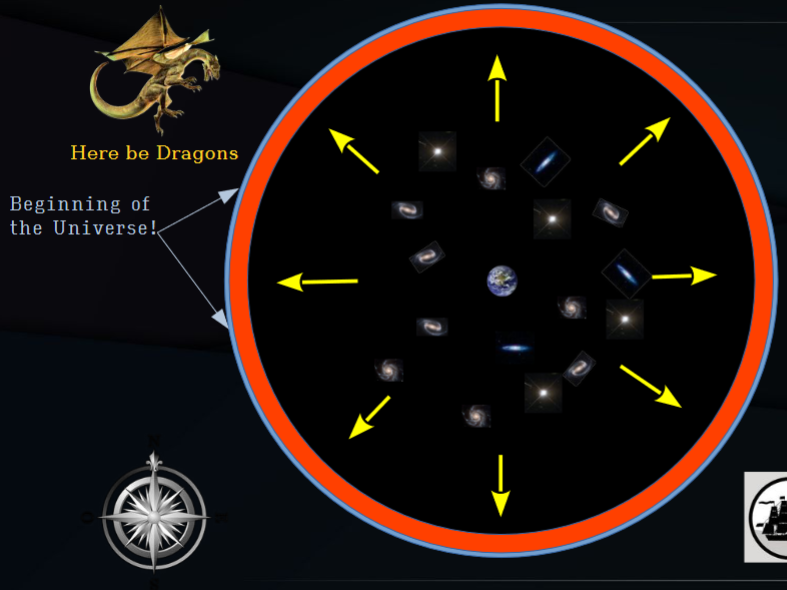
\includegraphics[width=0.8\textwidth]{universe}
            \caption{The universe (not to scale lol).}
            \label{fig:universe}
        \end{figure}
    \item the further away we look in the universe, the farther back in time we look
    \item the universe is expanding and cooling and is now transparent, but a long time ago, it was very hot and filled with plasma (blackbody) and was opaque 
    \item if we look far enough, we should be able to see what the universe looked like when it was filled with opaque plasma 
    \item the plasma is moving away from us at very close to the speed of light
    \item instead of seeing visible light, the light from the plasma has been doppler shifted down to the microwave region
    \item this is what we call the \textbf{Cosmic Microwave Background} 
    \item we have measured the spectrum coming from the night sky, and we see that it has the exact same spectrum as a blackbody curve -- nearly zero error
        \begin{figure}[h]
            \centering
            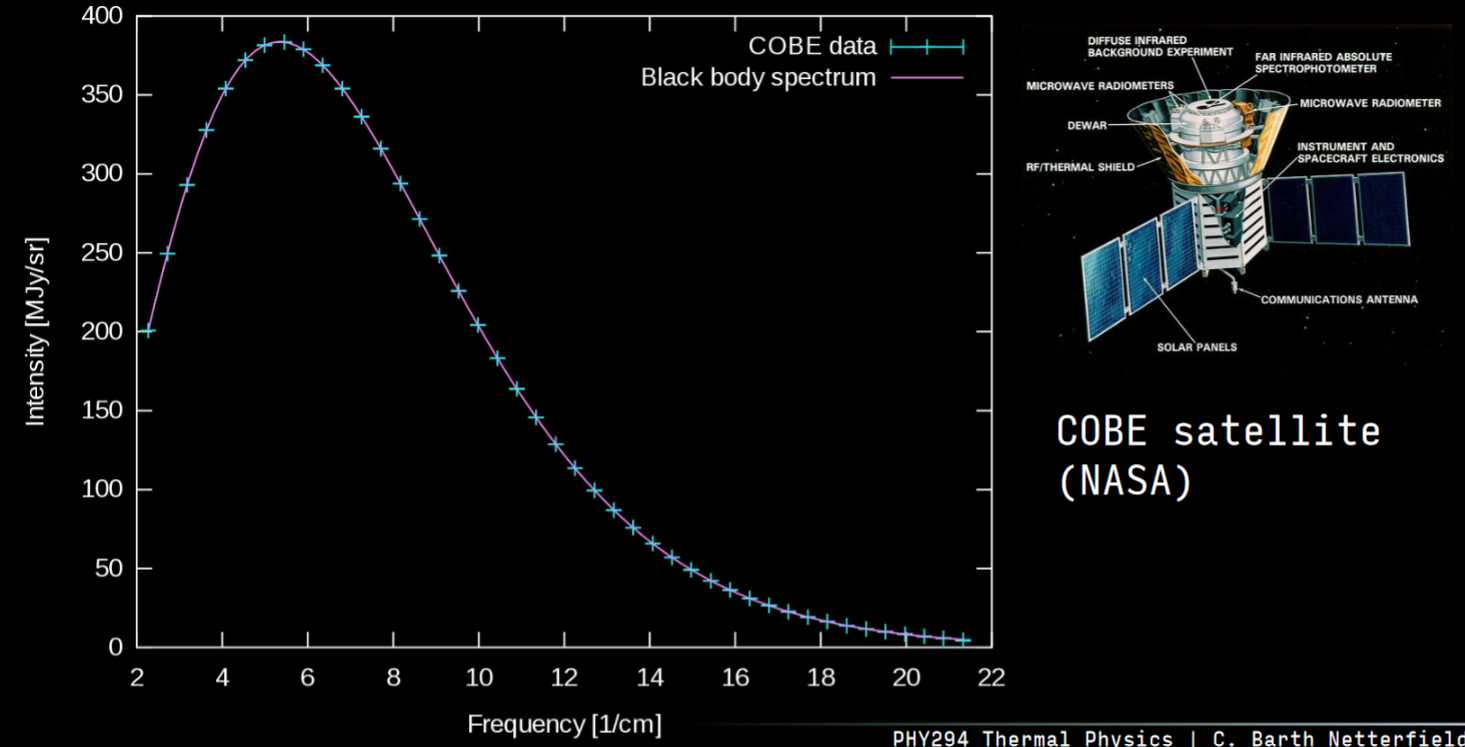
\includegraphics[width=0.8\textwidth]{cosmicMicroBackground}
            \caption{Spectrum of the Cosmic Microwave Background.}
            \label{fig:cosmicMicroBackground}
        \end{figure}
    \item point is: blackbody radiation is extremely important -- it was one of the huge proofs of quantum mechanics early on -- and it's crazy how it can be calculated using statistics
\end{itemize}




\section{Lecture 16 -- The Debye Theory}
\subsection{Heat Capacity of a Metal}
\begin{itemize}
    \item recall that we can calculate heat capacity through 
        \begin{gather*}
            C_V = \left( \frac{\partial U}{\partial T}  \right)_V
        .\end{gather*}
        where $U = \sum_{s} \epsilon_s \overline{n}$
    \item there are two ways to store energy in a metal:
        \begin{enumerate}
            \item the conduction electrons form a fermi gas 
            \item there are vibrational modes in the solid
        \end{enumerate}
    \item we first look at the heat capacity of the electrons by looking at the heat capacity of a fermi gas for $T>0$:
        \begin{itemize}
            \item we find that at low $T$, $C_V$ is proportional to $T$: 
                \begin{gather*}
                    C_V = \gamma T
                .\end{gather*}
        \end{itemize}
    \item we now look at heat capacity of vibrational modes:
        \begin{itemize}
            \item we can model the vibrations as acoustic waves (instead of using an Einstein solid since the vibrations aren't independent of each other)
            \item we define \textbf{phonons} as the acoustic modes in a solid:
                \begin{figure}[H]
                    \centering
                    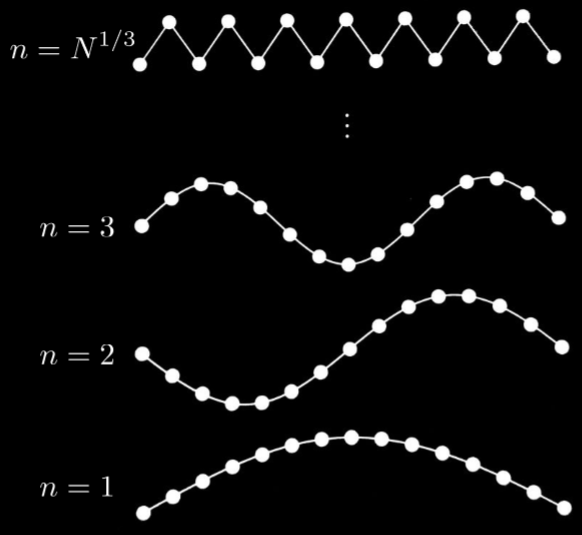
\includegraphics[width=0.5\textwidth]{phonons}
                    \caption{Phonons in a solid. Can think of them as the sound equivalent of photons.}
                    \label{fig:phonons}
                \end{figure}
            \item phonons have 3 "polarizations" (directions of vibration)
            \item after a lot of math and using the Debye approximation, we get that at low $T$, $C_V$ is: 
                \begin{gather*}
                    C_V = \frac{12\pi^4}{5} \left( \frac{T}{T_D} \right)^3 Nk
                .\end{gather*}
        \end{itemize}
    \item so at low temperatures: 
        \begin{gather*}
            C_V = \gamma T + \frac{12\pi^4 Nk}{5T_D^3}T^3
        .\end{gather*}
        where
        \begin{gather*}
            T_D \equiv \frac{\epsilon_0}{k} \left( \frac{6N}{\pi} \right)^{\frac{1}{3}} = \frac{hc_s}{2Lk} \left( \frac{6N}{\pi} \right)^{\frac{1}{3}}
        .\end{gather*}
        is the Debye temperature -- a function of the speed of sound and the size of the metal
    \item dividing through by $T$, we can rewrite the equation for heat capacity as
        \begin{gather*}
            \frac{C_V}{T} = \gamma + \frac{12\pi^4 Nk}{5T_D^3}T^2
        .\end{gather*}
    \item this tells us that plotting $C_V / T$ for different materials with respect to $T^2$ should produce a straight line with an intercept of $\gamma$ and a slope given by the coefficient of $T^2$, and it does:
        \begin{figure}[H]
            \centering
            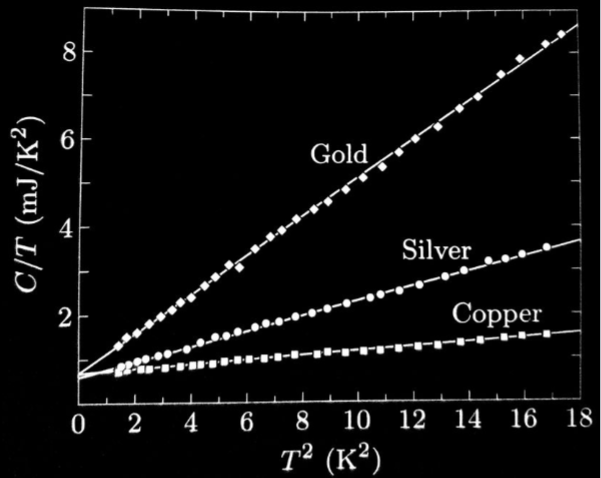
\includegraphics[width=0.6\textwidth]{CVSolid}
            \caption{$C_V / T$ vs $T^2$ for different metals.}
            \label{fig:CVSolid}
        \end{figure}
\end{itemize}



\section{Lecture 17 -- Bose Condensate}
\begin{itemize}
    \item previously we looked at fermions at low temperatures
    \item we now look at bosons at low temperatures
    \item as bosons, constrained to a small volume, are sufficiently cooled, they all end up in the ground state -- called \textbf{Bose Condensate} 
    \item consider a cold box of rubidium atoms (which are bosons)
    \item how many will be in the ground state?
    \item approach the problem by thinking about the occupancy of quantum modes (instead of the probability of a single particle being in a certain quantum mode)
    \item recall that the occupancy of a certain quantum mode is given by 
        \begin{gather*}
            \overline{n}_{BE}  = \frac{1}{e^{(\epsilon-\mu) / kT}-1}
        .\end{gather*}
    \item so just find $\mu$, plug it in, and find occupation
    \item example: for $N=10000, T = 100$ nK, we get a numerical solution of $\mu = 2.56952 \times 10^{-32}$
    \item plugging $\mu$ into the formula for occupancy, we get that the occupancy of the ground state is 7206 -- roughly 72\% of the particles are in ground state
    \item this shows us that bose condensates should form -- and they do!
    \item so for a quantum system:
        \begin{itemize}
            \item don't think about particles moving around described by quantum mechanics 
            \item instead think about quantum modes that may or may not be occupied 
            \item $N$ is conserved, but don't think of it as describing the number of 'objects', instead should be thought of as $N = \sum_{s} \overline{n}$
            \item the existence of bose condensates (among other things) show that this way of thinking is correct
        \end{itemize}
\end{itemize}







\end{document}








